\chapter{Desenvolvimento da Aplicação P.E.M.D.}
\label{Formulação do ambiente}


Os passos básicos para o desenvolvimento da ferramenta se apresentam simples, porém são extremamente complexos, sendo que inicialmente deve-se montar o histórico de mapas de quadrículas regionalizados, sendo tal etapa representado na seção \ref{Formulação do Ambiente}, que irá desenvolver e mostrar todos os passos utilizados para se chegar até o histórico de mapas de quadrículas regionalizados.

A função de previsão é apresentada em \ref{A função de previsão e a ponderação das matrizes de convolução}, seguindo um fluxo diferente do utilizado durante o desenvolvimento. Neste caso elaborou-se primeiramente a função de avaliação, imaginando como sua estrutura poderia ser modelada em uma função de previsão, facilitando assim diversas tentativas de se chegar na função de previsão apresentada. 

É apresentado em \ref{Aplicando o ICA} como estes mapas de quadrículas regionalizados são preparados para a utilização no ICA, que irá otimizar os parâmetros de previsão, e ainda como fora elaborada a função de avaliação utilizada para otimizar estes parâmetros. Também são descritos como os elementos do ICA genérico são utilizados e aplicados na modelagem do problema.

E por fim apresenta-se como a função de previsão foi modelada no P.E.M.D., apresentando um algoritmo detalhado de como a função de previsão fora programada e definindo como a aplicação combinou todos os elementos para gerar o mapa de previsão.


\section{Formulação do Ambiente}
\label{Formulação do Ambiente}

Iniciando-se com os dados de entrada utilizados para o desenvolvimento da solução, os quais, neste caso, representam e classificam, quando e onde ocorreram instalações na rede de distribuição elétrica de uma dada região. O objetivo é obter a partir destes dados a previsão de expansão espacial urbana, no caso, relativo à densidade de carga elétrica. Assim pode-se aplicar tal previsão no planejamento de cargas, em sistemas inteligentes de energia (smartgrids), gerenciamento de cargas (reposicionamento de transformadores ou subestações para localizações mais apropriadas), dentre outros. 

Para o desenvolvimento da metodologia de previsão de densidade espacial urbana (métricas da função de previsão) é necessária a análise de fatores que caracterizam um ou mais fatores de representação para densidade (tal que estes variem no tempo), e de fatores que representam o espaço em que estes fatores de densidade se aplicam. Isto quer dizer que, inicialmente, é necessário o uso de dados concretos baseados diretamente na posição geográfica em que o fator de densidade se encontra e evolui durante o tempo, de modo que a posição geográfica do fator represente, de fato, um ponto no espaço ao qual será prevista a evolução dos fatores de densidade durante um determinado intervalo de tempo.

Entende-se como fatores que representam o espaço em que os fatores de densidade evoluem, como sendo uma composição de fatores que possuem relação direta com o fator de densidade, de forma a representarem este fator de dentro de um plano espacial, que neste caso, são utilizados os pontos de latitude e longitude citados acima para representar a existência deste determinado fator (neste caso, a instalação de ponto da rede elétrica propriamente dita) dentro do espaço em questão. Então tem-se um espaço bidimensional formado por pontos de latitude (representado pelo eixo das ordenadas) e longitude (representado pelo eixo das abcissas), e limitado em latitudes e longitudes, máximas e mínimas, formando uma região retangular que contém tal representação dos fatores de densidade.

Ainda sem se preocupar com os fatores de densidade que se alteram durante o tempo, apenas focando nas posições geográficas que compõem os dados, faz-se o uso da filosofia de quadriculas \cite{willis2002spatial}, para tornar o espaço homogêneo, pois inicialmente, este espaço era representado por um conjunto de pontos espaçados desigualmente, de modo que seria muito custoso computacionalmente representar e processar todos os dados de forma a cumprir o objetivo apresentado por este trabalho.

Assim, é possível gerar um mapa de quadrículas homogêneas que representará os dados iniciais na forma de uma matriz, com a altura (número de linhas) sendo o número de quadrículas de norte a sul, e largura (número de colunas) como sendo o número de quadrículas de leste a oeste. Tal matriz pode ser usada para mapear uma região geográfica em uma matriz de dados que possa ser computada sem que seja preciso se preocupar com os fatores de localização geográfica, como por exemplo, converter ou calcular a distância entre 2 pontos geográficos, pois o espaço entre as quadrículas já é normalizado.

Para se fazer previsão de densidade espacial urbana é necessário que se modele um cenário no ambiente computacional, que seja capaz de representar com um certo nível de fidelidade, o que o ambiente real representa. Para criar tal ambiente computacional é preciso primeiro a geração ou obtenção de uma quantidade de dados os quais serão usados na modelagem deste ambiente. Os dados em questão referem-se a densidade de cargas, que é analisado em uma região urbana de forma espacial. 

A base de dados utilizada para fazer a previsão de densidade de carga espacial urbana representa uma estimativa das datas de instalação de pontos de rede elétrica  durante um período de tempo e de uma determinada região e, portanto são dados que variam no tempo. Os pontos de instalação elétrica foram classificados em residencial, residencial de baixa renda, comercial, industrial, público e rural. Inicialmente imaginou-se que pontes, ruas, rios, altitude, inclinação, etc. poderiam ser úteis como dados de atração, representando pontos que não variam em pequenos intervalos de tempo, e portanto, fixos durante todos os períodos, porém foram removidos para que a análise ficasse mais limpa, pois estavam gerando ruído nos resultados e acumulando muito erro durante a previsão. Então, cada ponto de instalação elétrica possui um município, um grupo, uma data de criação e valores que definem sua localização geográfica, representados por valores numéricos reais de latitude e longitude. Com estes dados separados é possível então criar um banco de dados para armazenar toda informação que é captada, gerada ou obtida, normalizando assim toda entrada de dados para a aplicação apenas nestas 5 características.

Com a tabela possuindo um número grande de dados durante os períodos, é possível separar estes dados em diversos mapas matrizes (mapas de quadrículas) representando a quantidade de carga instalada em cada região e sua evolução durante um período de tempo. A quantidade de mapas é definida pelo intervalo de tempo que se deseja processar. Por exemplo, se inicialmente foram obtidos dados nos períodos entre 2005 até 2015, e o período de tempo desejado é de um ano, geram-se então, 10 mapas matrizes de densidades de carga onde cada mapa matriz possui a densidade de carga para cada período, neste caso, para cada ano.

Antes de gerar os mapas matrizes, ainda é necessário mais um passo, que é a criação de arquivos, a partir do banco de dados, onde cada arquivo representa o período em que se deseja obter os mapas matrizes. Para isto, foram criados diversos filtros no banco de dados para cada período, onde cada filtro seleciona todas as linhas que estejam dentro do intervalo de duas datas, uma inicial e outra final, sendo que destas duas datas, a data inicial é referente sempre a data do período inicial, e a segunda é referente ao período em questão, pois os dados devem representar valores crescentes, e não a diferença entre os períodos. Outra funcionalidade que cada filtro aplica nas linhas, é a adição de um valor de contagem, denominado “Total”, para cada ponto de coordenada geográfica que possa ter sofrido crescimento, sendo este aumento referente a mais instalações de pontos de rede elétrica nesta mesma coordenada, como por exemplo a construção de um prédio, residência ou qualquer outro tipo de adição que possa vir a representar uma forma de crescimento de consumo de carga para aquela coordenada. Assim, cada arquivo deve ser salvo em modo texto, possuindo os nomes seguindo a seguinte forma, \(“<período0>.csv”, “<período1>.csv”, ..., “<períodoN>.csv”\), e ainda dentro dos arquivos, os dados serão filtrados de modo que transformem a tabela inicial em uma tabela contendo os campos: Longitude, Latitude, Grupo e Total.

Toda a modelagem dos dados de carga citados anteriormente ocorreram fora da aplicação, e foi utilizada a ferramenta \(sqlite\) para a criação, armazenamento e filtragem dos dados para a utilização destes na aplicação. Já na aplicação, a primeira definição que deve ser feita é sobre a região que se deseja utilizar, sendo esta definida por valores de longitude, leste e oeste, e valores de latitude, norte e sul. Com estes quatro valores formando um setor terrestre quadrangular, onde tal setor representa a região que se deseja processar para obter a previsão espacial de carga. Os dados presentes nos arquivos gerados para cada período que estiverem fora destes intervalos de (norte, sul e leste, oeste) serão ignorados, sendo apenas processados os dados dentro dos intervalos citados. 

Os valores presentes nos arquivos de período ainda não estão discretizados, para que possam ser processados  mais homogeneamente, então, utiliza-se a técnica de quadriculamento do setor para discretizar as regiões de forma a fazer com que o mapa seja particionado em tamanhos iguais e, consequentemente cada parte igual do mapa receba um valor de carga de acordo com aquela região. Assim, forma-se um mapa, denominado \(Mapa Matriz\), para cada período, que representa a densidade de carga espacial em porções homogêneas.

A segunda definição deve ser o tamanho de cada quadrícula, que é definida a partir de apenas um valor numérico, que representa o tamanho dos seus lados em metros. Com estas duas definições iniciais pode-se então criar um mapa de quadrículas que será usado posteriormente como base para a geração dos mapas matrizes. 
	
O mapa de quadrículas utiliza-se destes 5 valores iniciais para ser gerado, e nele definem-se as quantidades de quadrículas que irão compor o mapa em altura e largura, e consequentemente a quantidade de quadrículas total do mapa, que pode ser calculado multiplicando a altura com a largura. Os valores de altura e largura são calculados em duas etapas, onde a primeira etapa fornece a largura/altura total em metros e a segunda etapa resolve a quantidade de quadrículas para altura e largura, dividindo os valores de altura e largura totais em metros pelo tamanho de cada quadrícula em metros, como pode ser visto nas equações \ref{eq:building-matrix-map-one} e \ref{eq:building-matrix-map-two}:

\begin{equation}
\label{eq:building-matrix-map-one}
\begin{split}
widthInMeter = Abs(DistanceTo(north, east, north, west));\\
heightInMeter = Abs(DistanceTo(north, east, south, east));
\end{split}
\end{equation}

\begin{equation}
\label{eq:building-matrix-map-two}
\begin{split}
mapWidth = widthInMeter / quadricSizeInMeter;\\
mapHeight = heightInMeter / quadricSizeInMeter;
\end{split}
\end{equation}

A chamada função \(DistanceTo\) calcula a distância em metros entre dois pontos de coordenadas geográficas quaisquer utilizando a fórmula de haversine \cite{shumaker1984astronomical}, \cite{snyder1987map}, onde os dois primeiros valores representam o primeiro ponto e coordenada geográfica e os últimos dois valores representam o segundo ponto de coordenada geográfica. Observa-se que na primeira chamada, mantiveram-se os pontos de latitude fixos em norte, de forma a deslocar-se apenas horizontalmente (de leste para oeste) e na segunda chamada mantiveram-se fixos os pontos de longitude fixos em leste, de forma a deslocar-se apenas verticalmente (de norte para sul), para assim obter o valor transformado de coordenada geográfica para coordenada cartesiana em metros, para largura e altura respectivamente.

Com a quantidade de quadrículas para altura e largura calculados para o mapa de quadrículas, agora é preciso popular cada índice do mapa com uma quadrícula. Cada quadrícula é representada por um ponto de coordenada geográfica, composto por latitude e longitude, podendo este ser convertido em uma distância a partir do ponto inicial ou em um ponto de utm (que é o ponto de coordenada geográfica representado pela \emph{Universal Transversa de Mercator}). Então, para isto, são necessárias mais duas definições, um ponto inicial e uma direção de iteração. 

O ponto inicial pode ser definido como qualquer combinação dos valores de latitude e longitude dados inicialmente, então, pode-se ter o ponto inicial como sendo\( (Norte, Leste)\), \((Norte, Oeste)\), \((Sul, Leste)\) ou \((Sul, Oeste)\), porém deve-se prestar atenção em definir a direção como sendo a oposta ao ponto inicial, uma vez que o processo de inicialização do mapa de quadrículas já possui seus limites definidos e a direção é quem define para qual sentido serão geradas as quadrículas (iterando-se em altura e largura) a partir do ponto inicial. Então, por exemplo, se o ponto inicial for \((Norte, Leste)\), a direção de crescimento deve ser representada pelo texto \(“so”\), assim, tem-se uma iteração que gera quadrículas dentro dos limites do mapa de quadrículas, que vai de Norte para Sul e de Leste para Oeste. Caso a direção de crescimento para o mesmo ponto do exemplo seja outra, digamos, \(“sl”\), o mapa terá como ponto inicial os pontos definidos como Norte e Leste, crescerá de norte a sul, porém de Leste a leste, tendo um deslocamento para fora dos limites do mapa de quadrículas esperado, o que pode implicar em um preenchimento incorreto do mapa matriz, que define as cargas, nos próximos passos da aplicação.
	
Finalizando a criação do mapa de quadrículas, ainda são definidos 5 valores e uma função, sendo estes, o Ponto Final, que representa o ponto mais distante ao ponto inicial, tendo sua distância como a diagonal principal do mapa de quadrículas, e os valores para Latitude Máxima, Longitude Máxima, Latitude Mínima, e Longitude Mínima, definidos a partir dos pontos inicial e final. Estes últimos 4 valores, são usados pela função a ser definida, que, por sua vez, calcula os índices \((x,y)\) do mapa de quadrículas, a partir de um ponto de coordenada geográfica (Latitude, Longitude), isto é, dado um ponto na forma (Latitude, Longitude), a função deve retornar em qual quadrícula do mapa de quadrículas (mapa matriz) este ponto se encontra. Esta é uma função usada para preencher os mapas matrizes a partir dos dados nos arquivos de períodos.

Com o mapa de quadrículas criado, inicializado e seus valores propriamente definidos dentro dos limites estipulados (Norte, Sul, Leste, Oeste), sua estrutura pode ser ilustrada como apresentada na Figura \ref{fig:Ilustrations-QuadricMap}: 


\begin{figure}[h]
	\centering
	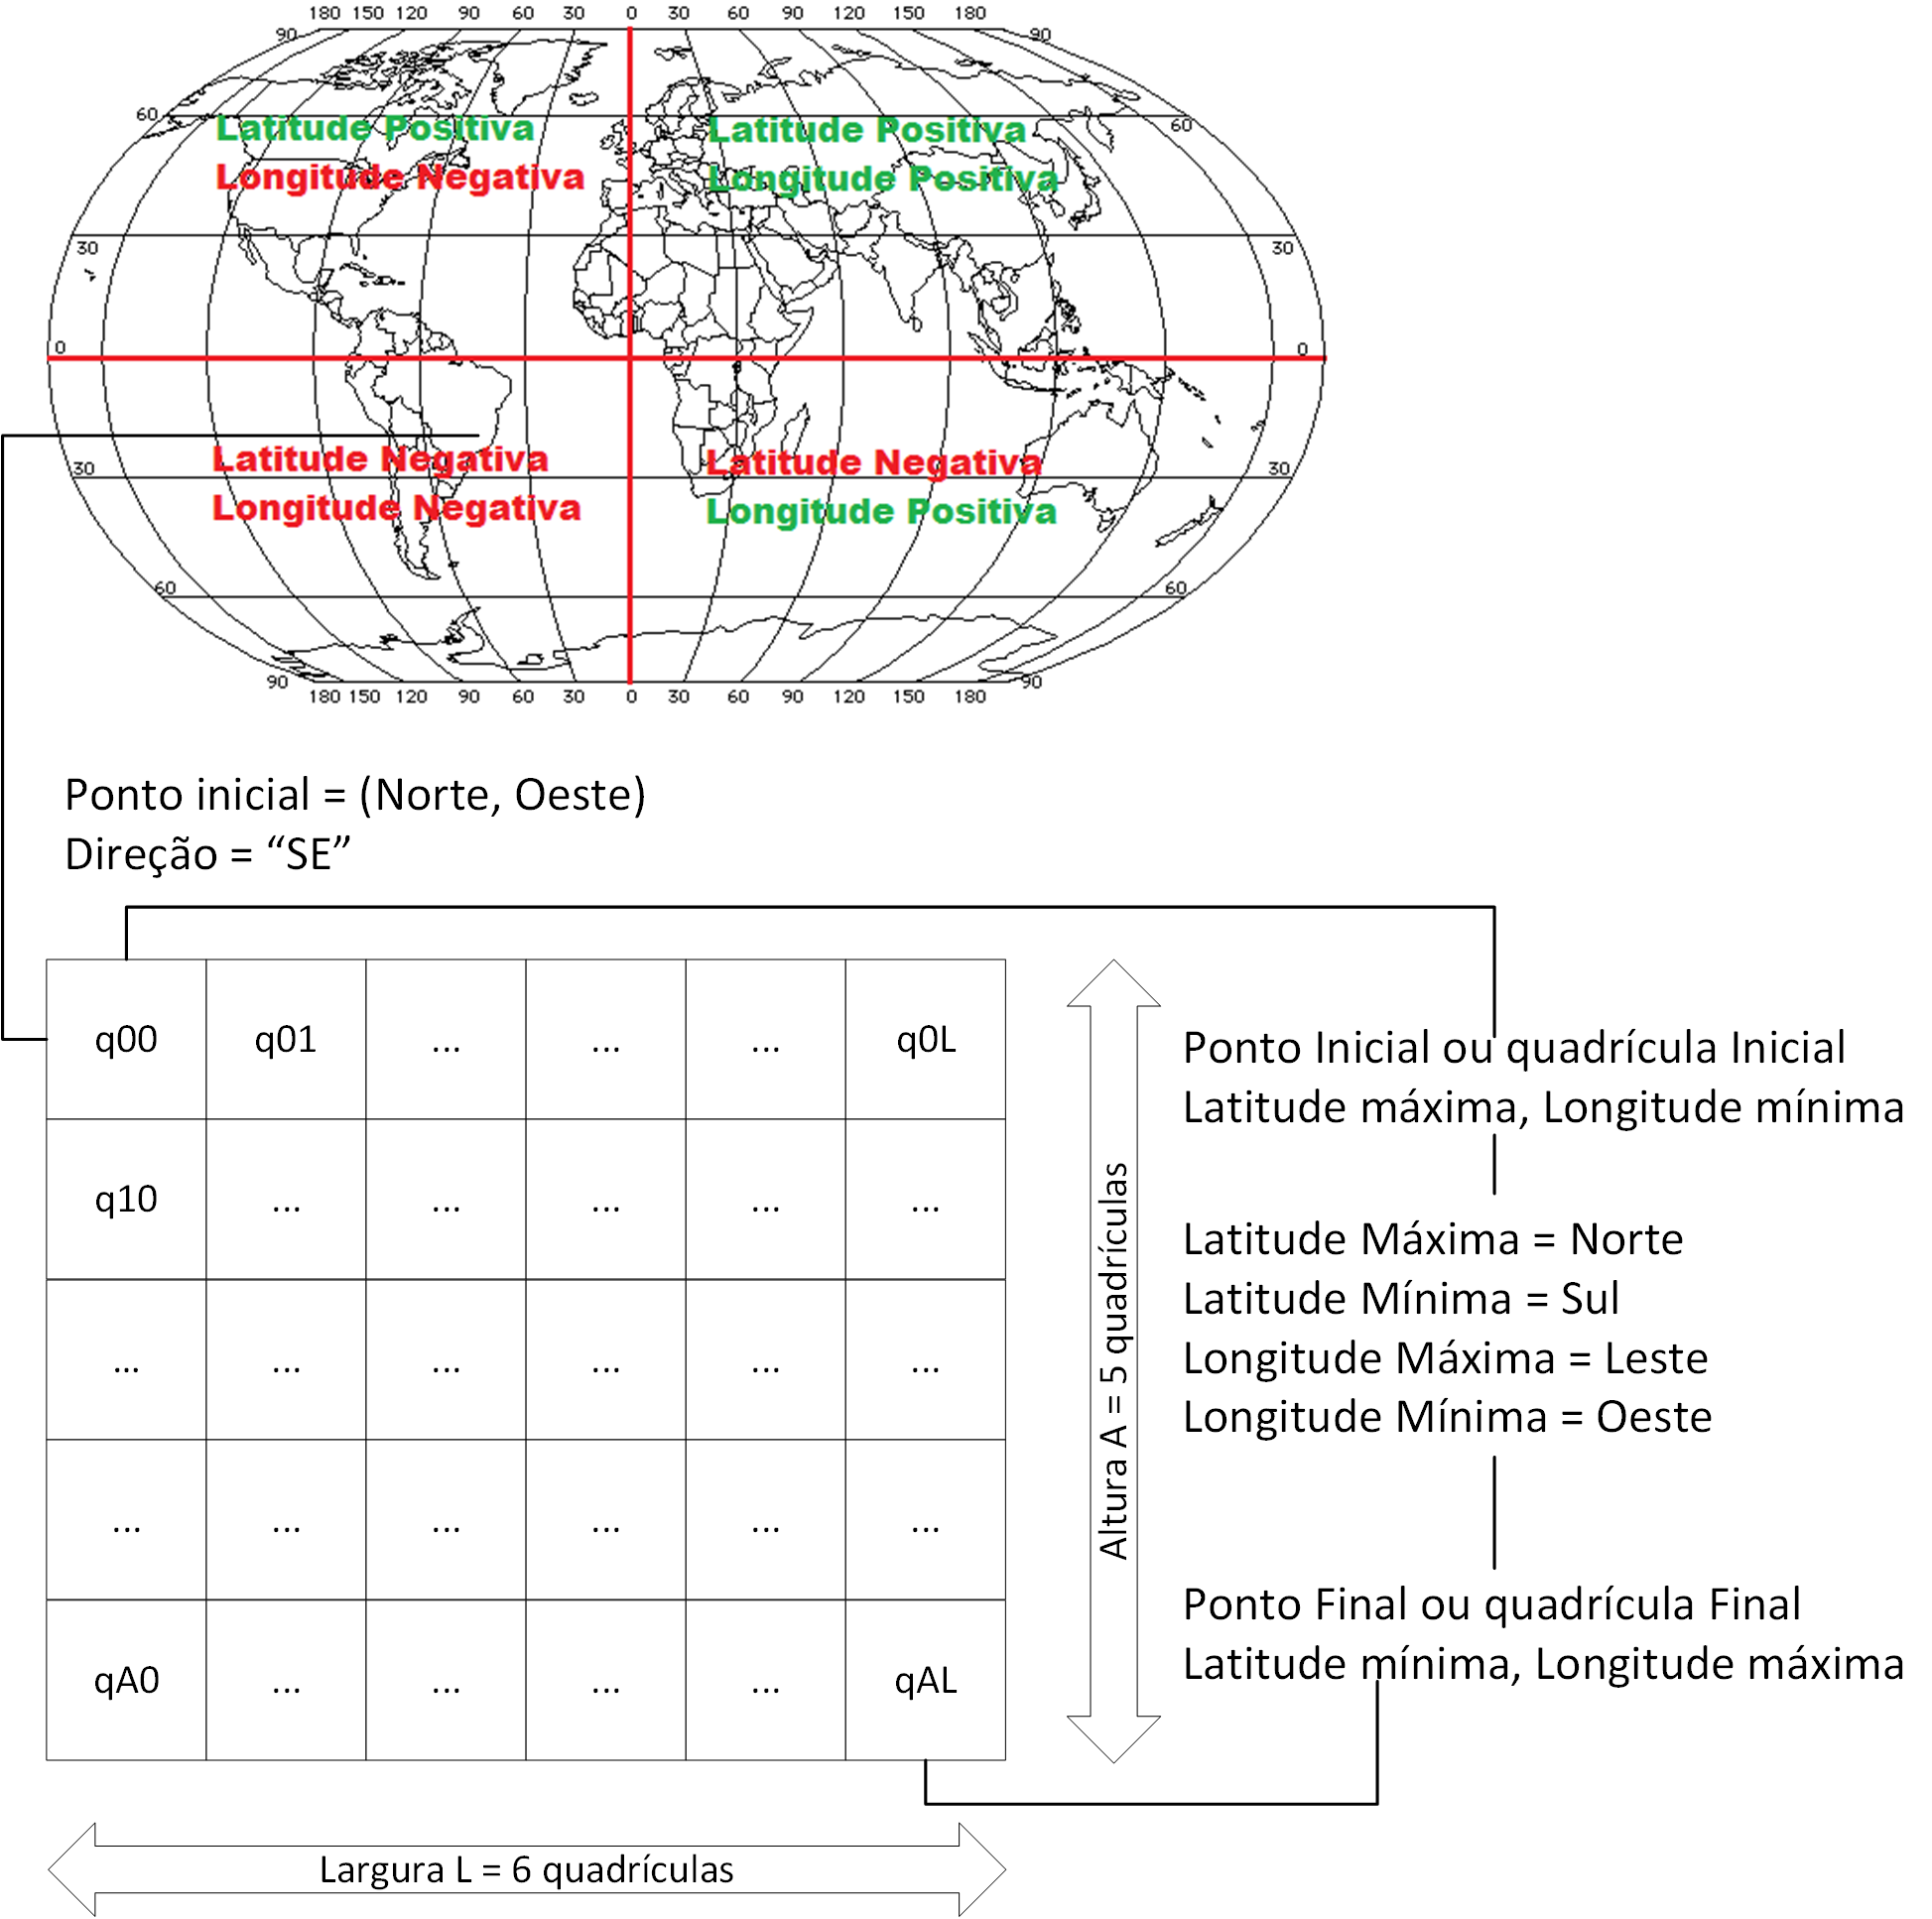
\includegraphics[scale=0.6]{Figuras/Ilustrations-QuadricMap.png}
	\caption{Ilustração da montagem do mapa de quadrículas.}
	\label{fig:Ilustrations-QuadricMap}
\end{figure}


Observe a região escolhida está no hemisfério sul a esquerda do meridiano de \emph{Greenwich}, o que indica que os valores para latitude e longitude (em graus) sempre serão negativos, e assim, de acordo com a posição inicial e a direção escolhida, os valores máximos para latitude e longitude se resolvem como apresentado.

Passando agora para os mapas matrizes, que nada mais são que uma lista de matrizes com o mesmo tamanho, em altura e largura, do mapa de quadrículas, e tal que a quantidade de mapas matrizes é referente a quantidade de períodos. Cada índice de um dado mapa matriz é diretamente mapeado para uma quadrícula do mapa de quadrículas, podendo assim, este mapa matriz representar um mapa de densidades genérico, sem relação direta ao mapa de quadrículas, porém pode-se usar o mapa de quadrículas para localizar e dar sentido ao mapa matriz sempre que necessário. 

Tal encapsulamento dos valores de densidade em uma lista de mapas matrizes, de tamanhos iguais, e de forma que seus índices representem valores de densidade, os quais são crescentes de acordo com o período de cada mapa matriz, faz com que a aplicação seja capaz de processar qualquer mapa de densidades sem se 'preocupar' com a localização geográfica real que este mapa matriz representa. O mapa de quadrículas então, tem duas funcionalidades básicas, que é a de inicializar a região a partir dos dados iniciais, e abstrair as informações geográficas para os mapas matrizes, os quais representam as densidades de carga em cada período.

A partir do mapa de quadrículas gerado e o conceito dos mapas matrizes, pode-se então, escolher qualquer fator para inserir em seus índices, como por exemplo, pode-se criar um mapa de quadrículas para uma determinada região tal que o fator escolhido sejam valores de altitude ou de inclinação. Porém para que uma previsão seja feita é necessário utilizar dados de densidade que variam de acordo com o tempo, como é o caso dos dados citados no início desta seção, os quais podem ser mapeados em vários mapas matrizes cada um representando um período de tempo diferente e diferenciados pelo mesmo intervalo de tempo, como por exemplo, poderia ser gerado um mapa de quadrículas do total de instalações elétricas até 2010, um até 2011 e assim por diante.

Sabe-se que os fatores de densidade devem estar diretamente relacionados com os valores de posição geográfica, por isto podem ser inseridos em qualquer mapa de matriz, e que também, devem variar no tempo, para que possam ser gerados diversos mapas de matrizes, com cada fator representando assim, um período de tempo bem definido e espaçados no tempo uniformemente, tal que possam ser geradas previsões futuras à estes períodos e de mesmo intervalo de tempo.

Neste trabalho, ainda não foi modelada a previsão de múltiplos fatores, mas já foi elaborada uma estrutura que converge vários fatores de carga para apenas um fator de densidade de carga, denominado “multiplicadores de carga”.

Para a criação da lista de mapas matrizes, é então, utilizado o mapa de quadrículas já processado, os arquivos de períodos e uma estrutura que representa a densidade de carga de cada tipo de região, denominada “multiplicadores de carga”. Para este trabalho foram consideradas as regiões do tipo residenciais (\(m=1\)), comerciais (\(m=3)\), industriais (\(m=10\)), residencial de baixa renda (\(m=0.5\)), rural (\(m=0.5\)), iluminação pública (\(m=1\)), sendo os valores de \(m\) o valor que irá multiplicar aquele tipo de carga ao montar o mapa de quadrículas. Assim, os mapas matrizes são preenchidos um a um, de modo que para cada linha do arquivo de período, busca-se qual o índice \((x,y)\) no mapa de quadrículas, através dos valores de latitude e longitude, então, com o índice \((x,y)\) seleciona-se o índice \((x,y)\) do mapa matriz e atribui a este índice, o multiplicador de carga referente ao Grupo da linha multiplicado pelo Total da linha, como mostra a expressão \ref{eq:MultiplicadorTipo}:

\begin{equation}
\label{eq:MultiplicadorTipo}
\centering
\begin{split}
(x,y) = MapaQuadrículas.BuscaÍndice(linha.Lat,linha.Long);\\
MapaMatriz(x,y) = MapaMatriz(x,y) +\\ MultiplicadorCarga[linha.Grupo] *\\ linha.Total;
\end{split}
\end{equation}
 
Este processo ocorre para cada linha de cada arquivo de períodos, e no fim da leitura de cada arquivo tem-se um mapa matriz que representa a região no mesmo período do arquivo. E por fim, todos os mapas matrizes gerados são adicionados em uma lista sequencial referente aos períodos.

Com a lista de mapas matrizes calculada, pode-se então definir um vetor que represente o crescimento absoluto entre cada período, fazendo a diferença entre o mapa matriz do período \(t\) com o mapa matriz do período \(t+1\), tendo assim, os valor de crescimento de \(t\) para \(t+1\), de \(t+1\) para \(t+2\), de \(t+p-1\) para \(t+p\), sendo \(p\) o número total de períodos selecionados. Assim o vetor é representado pela expressão \ref{eq:CrescimentoAbs}:

\begin{equation}
\label{eq:CrescimentoAbs}
\begin{split}
CrescimentoAbs =& \\
&\begin{bmatrix}
\\ mapaMatriz[t] - mapaMatriz[t+1], 
\\ mapaMatriz[t+1] - mapaMatriz[t+2], 
\\ ...,
\\ mapaMatriz[t+p-1] - mapaMatriz[t+p]
\end{bmatrix}
\\ 
\\ &0<t<(p-1),
\\ &p = número \  total \ de \ períodos. 
\end{split}
\end{equation}

Após o cálculo dos crescimentos absolutos entre os anos, particiona-se os mapas matrizes em partes menores, resultando assim em uma lista de mapas matrizes particionados. Tal particionamento se dá porque a operação que fará a otimização das estruturas para a previsão funciona melhor para pequenas porções, uma vez que quando se usa mapas muito grandes, a tendência é se aproximar da média de crescimento geral para aquela regão. A Figura \ref{fig:PartitionedQuadricMap} ilustra a estrutura de partições de mapas para partições de tamanho \(2X2\) e durante quatro períodos. Observe ainda na mesma figura, que o número de partições não ignora partições incompletas, usando-as assim, como regiões válidas para o processamento.

\begin{figure}[h]
	\centering	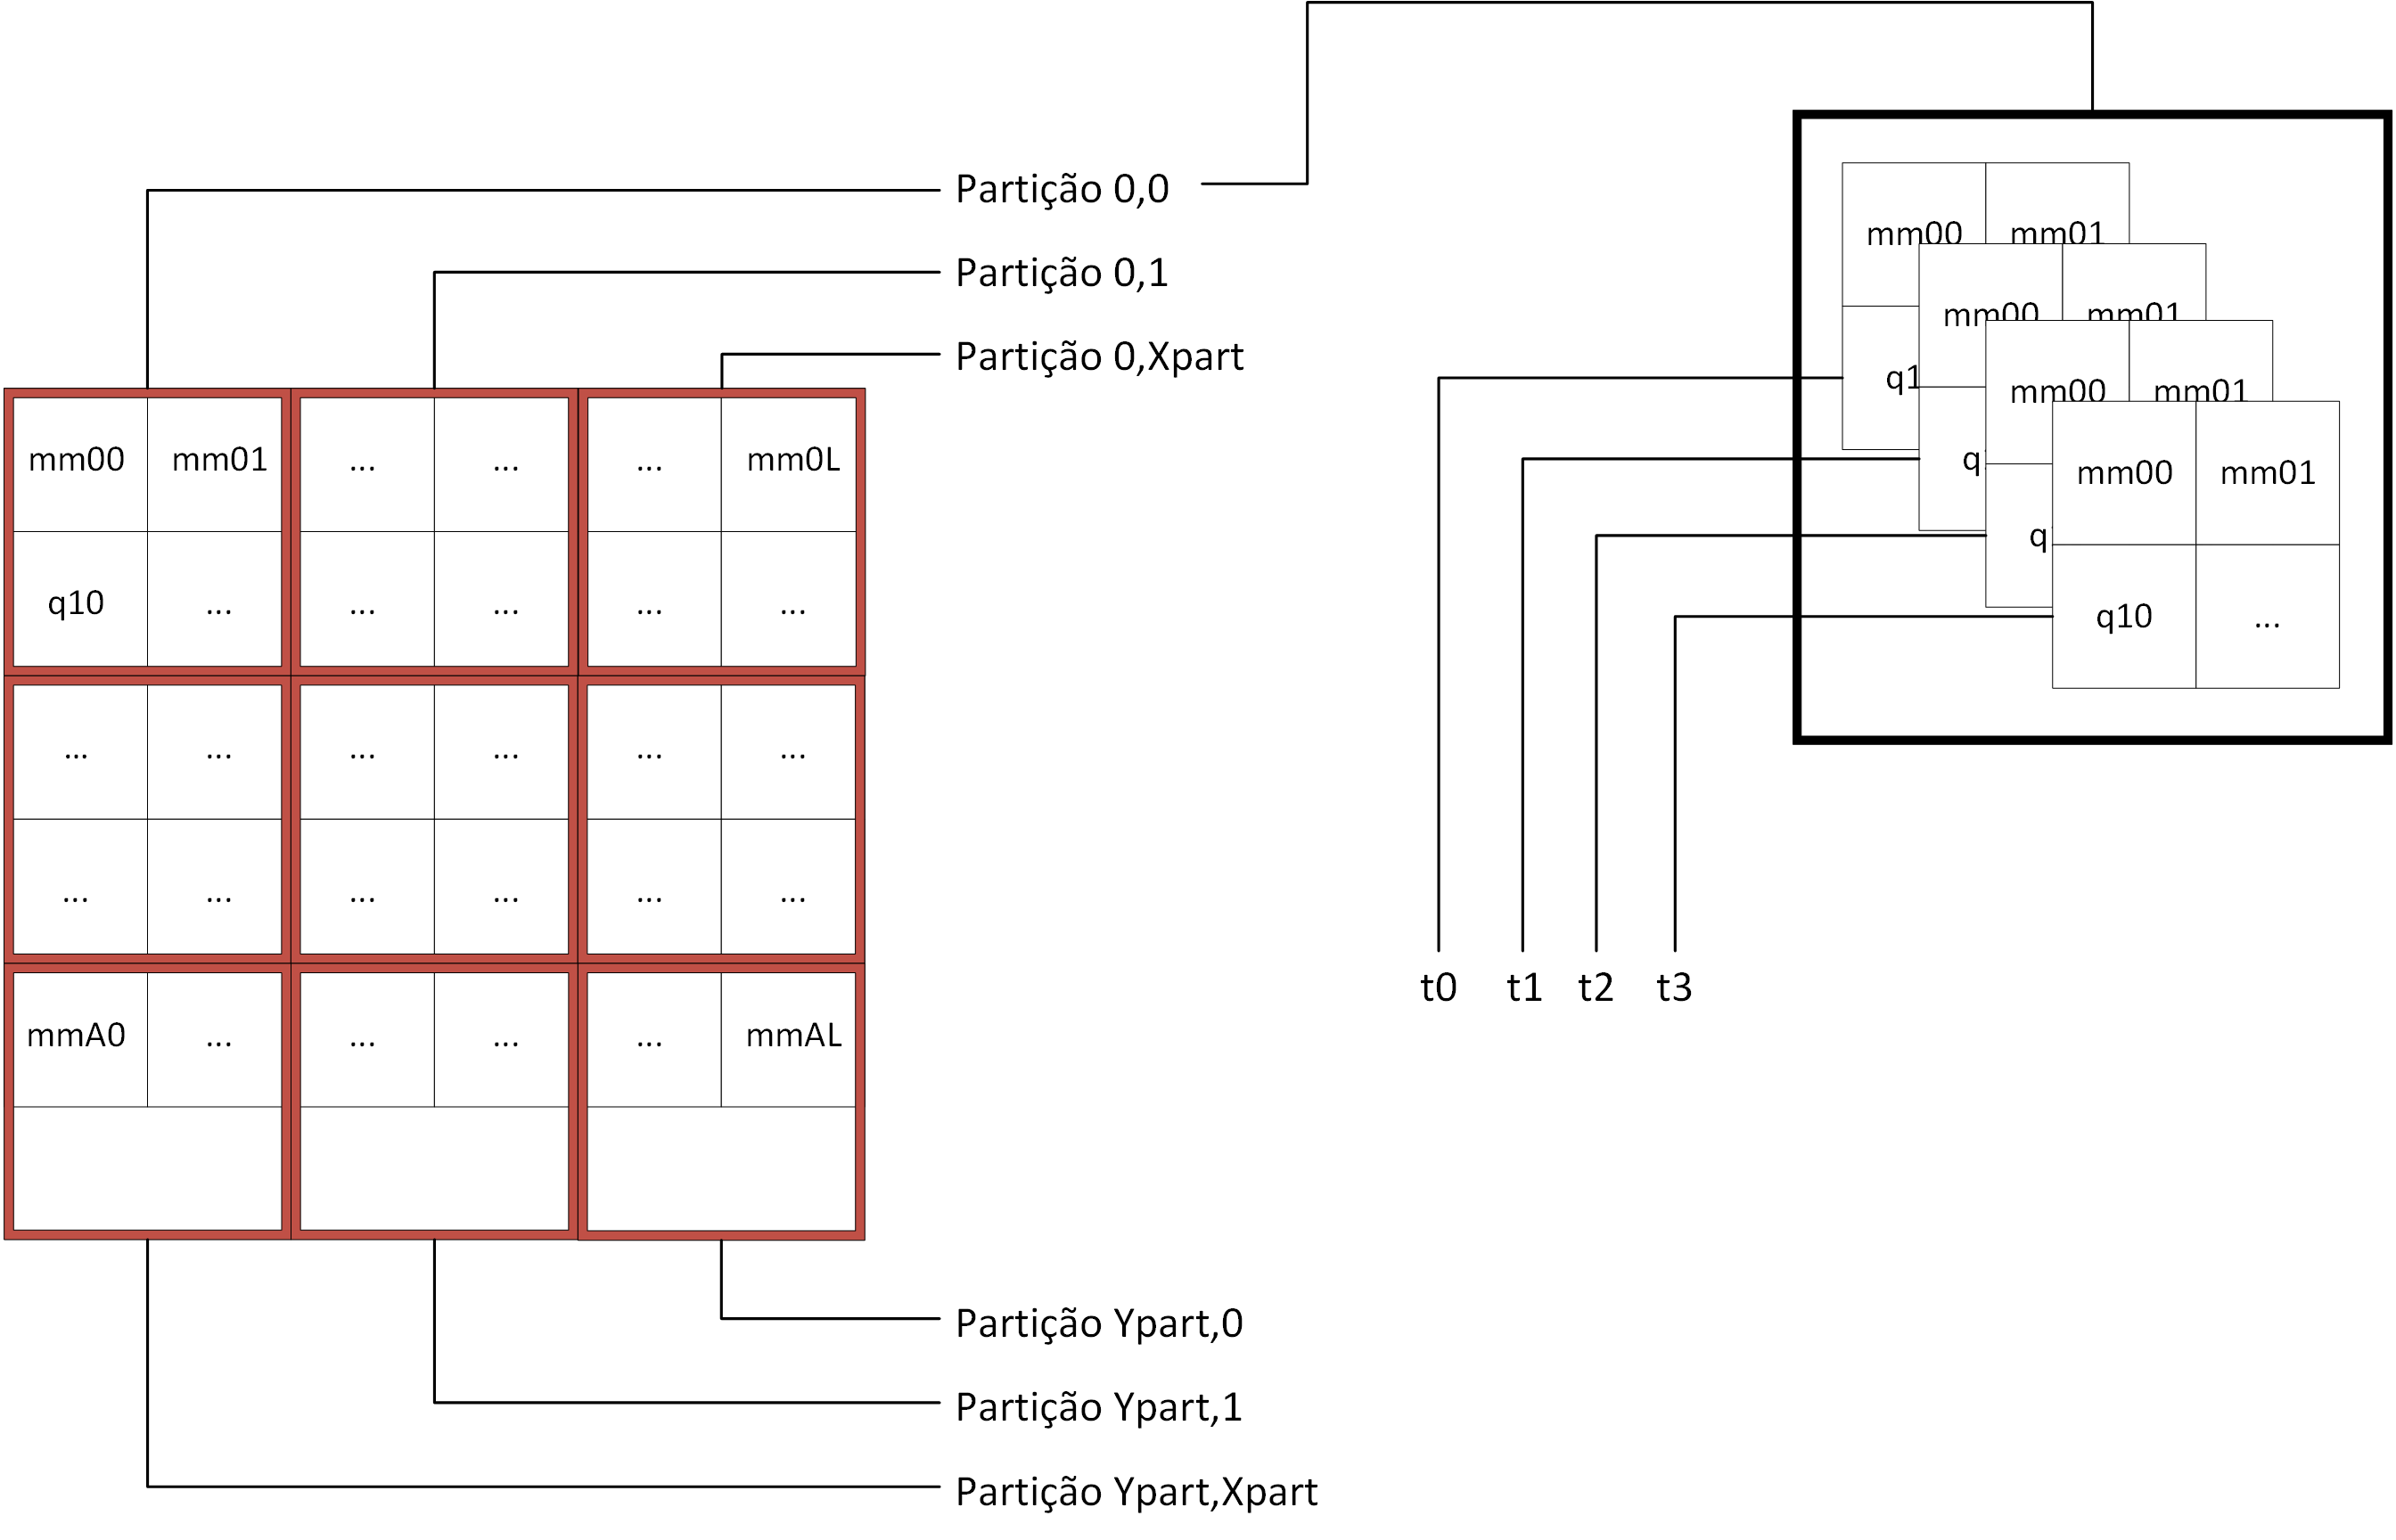
\includegraphics[scale=0.6]{Figuras/Ilustrations-PartitionedQuadricMap.png}
	\caption{Ilustração do mapa de quadrículas particionado.}
	\label{fig:PartitionedQuadricMap}
\end{figure}

Como mencionado nos parágrafos anteriores, este particionamento  é uma forma de fazer uma previsão sobre das pequenas regiões particionadas do mapa original, pois a operação de avaliação utilizada, é uma heurística que leva em consideração a operação de convolução sobre imagens, e neste caso, cada quadrícula está sendo representada por um pixel da imagem (mapa matriz) a ser operada pela convolução para gerar a previsão. Tal técnica será discutida mais adiante, mas já se adianta que a convolução tem a capacidade de  transformar uma matriz em outra, passando um filtro ou máscara de convolução sobre da matriz em questão, gerando uma matriz resultado. Caso se tente buscar um filtro de convolução para a matriz completa, englobam-se muitas características das áreas ou regiões mais influentes, e as regiões menos influentes serão ignorados. Isto resulta  apenas em um mapa que é a média da distribuição de carga geral por todo o mapa, e com um acúmulo de erro muito grande sobre os períodos, e que neste caso não nos interessa. Por este motivo é que foi feito o particionamento do mapa de modo que cada pequena região tenha destacada suas características principais a fim de fazer uma previsão mais precisa para todo mapa a partir da previsão das pequenas regiões. Este particionamento pode ser considerado um quadriculamento do mapa de quadrículas, o motivo pelo qual não se usa  uma quadrícula maior é que ela é usada segundo \citeauthor{willis2002spatial} \cite{willis2002spatial} com seu tamanho original de aproximadamente \(\frac{1}{4} milha\),  e para este trabalho, foi usado um tamanho menor, uma vez que se deseja ter mais resolução nos dados para a adição deste a mais, que particiona o mapa de quadrículas em vários mapas menores. Assim cada  partição é um conjunto de quadrículas que representará uma imagem a ser processada pelo algoritmo, o qual buscará a melhor previsão desta pequena região.

Então, ao final do processamento não se terá apenas uma solução para previsão  total do mapa, mas sim várias soluções boas de previsão, para várias pequenas regiões, as quais irão compor o mapa final de previsão para a quantidade de períodos escolhida.

Para se criar as partições inicialmente define-se apenas dois valores, que representará quantas partições haverão no eixo das ordenadas \(Xpart\) e no eixo das abscissas \(Ypart\). Assim, calcula-se o total de partições como sendo \(Xpart \cdot Ypart\). No caso da Figura \ref{fig:PartitionedQuadricMap}, \(Xpart\) e \(Ypart\) são iguais a 3. Assim como para o mapa final, cada partição será processada independente uma da outra, de modo que exista no final, uma previsão para cada partição dos mapas matrizes, as quais são reconstituídas em um único mapa matriz após todo o processamento para a apresentação do resultado final. Observe que como \(Xpart\) e \(Ypart\) são iguais a 3, cada partição tem o tamanho de 2, pois a regra de cálculo para o tamanho de cada partição a partir de \(Xpart\), \(Ypart\) segue a expressão \ref{eq:calcParts}:

\begin{equation}
\label{eq:calcParts}
\centering
\begin{split}
PartWidth = FLOOR(mapWidth / Xpart);\\
PartHeitht = FLOOR(mapHeight / Ypart);
\end{split}
\end{equation}

Calcula-se então os crescimentos absolutos para cada partição a fim de que este valor seja usado também pela função de avaliação que será utilizada no processo evolutivo, e armazena os valores em uma lista de vetores de crescimentos absolutos para cada partição. 

Conclui-se então, a modelagem do ambiente, demonstrando como os dados iniciais foram transformados até antes de serem processados para geração da previsão através do processo evolutivo, que neste caso será feita pelo algoritmo imperialista competitivo, com uma função de aptidão ou \emph{fitness} modelada utilizando os dados de uma lista de mapas matrizes particionado e os dados de crescimento absoluto nesta partição que serão descritos a seguir. Neste ponto os dados que aplicação possui carregados em memória são:
\begin{enumerate}
\item Mapa de quadrículas, carregado a partir dos arquivos gerados por seleção no banco de dados para cada período.
\item Vetor Multiplicador de Carga, definido de forma constante na aplicação. Para trabalhos futuros pode ser definido um multiplicador de carga para cada região particionada e seus valores podem ser definidos de acordo com algum algoritmo inteligente que processo os dados
\item Norte, Sul, Leste e Oeste, que são os limites em coordenadas que define a região da previsão.
\item Tamanho da quadrícula, em alta resolução, diferente do valor definido por \citeauthor{willis2002spatial}, de aproximadamente \(\frac{1}{4} milha\).
\item Vetor de períodos, não foi mencionado no texto mais quando se carrega os dados é criado um vetor contendo o valor de cada período apenas para impressão dos resultados  e definição dos períodos de treino e teste descritos posteriormente.
\item Uma lista de mapas matrizes, onde a quantidade de mapas matrizes presentes na lista é a quantidade de arquivos de períodos lidos no início da aplicação, e cada mapa matriz representa a densidade de carga em uma região durante o período que gerou este mapa matriz.
\item \(Xpart\) e \(Ypart\), que definem em quantas partições os mapas matrizes  serão quebrados para gerar uma previsão para cada conjunto de mapas matrizes de cada  uma destas partições.
\item Uma lista de mapas matrizes particionados, onde a quantidade de mapas matrizes particionados é igual a \(Xpart \cdot Ypart\),  e, para cada mapa matriz particionado será gerada uma previsão. 
\end{enumerate}




\section{A função de previsão e a ponderação das matrizes de convolução}
\label{A função de previsão e a ponderação das matrizes de convolução}

Espera-se que uma função de previsão forneça previsões certeiras sobre uma dada região. Assim, tal função deve levar em consideração duas formas básicas de parâmetros de entrada, sendo a primeira uma informação base para se gerar uma previsão, como um mapa de quadrículas de um período \(t_n\). O segundo tipo de parâmetros devem ser os parâmetros que irão alterar o primeiro parâmetro afim de que este se torne um mapa previsto de um período, digamos \(t_{n+1}\). Sendo assim, a função de previsão pode ser vista como algo do tipo \ref{Funcaodeprevisaobase}:

\begin{equation}
\label{Funcaodeprevisaobase}
t'_{n+1} = F(t_{n+1}, [p_0,p_1,p_2,...,p_n])
\end{equation}

Foi elaborada uma função de previsão baseada em convolução. Inicialmente almejava-se criar uma função que utilizasse apenas uma matriz de convolução como sendo os parâmetros desta função, afim de obter as características da evolução do histórico de mapas. Porém esta ideia foi frustrada pelo fato de que a utilização de apenas uma matriz de convolução, seja de qual ordem for, propaga muito erro para as previsões futuras. Assim, propõe-se uma função de previsão que faça uma ponderação entre diversas matrizes de convolução junto de alguns fatores de ponderação para que as características sejam propagadas para mapas futuros com menos erros, o que leva a um acerto maior na previsão. 

A ponderação se faz importante porque neste caso, as partições dos mapas que representam os períodos subsequentes, não necessariamente são o resultado da convolução de uma máscara pela região do mapa do período anterior. Então, deve-se estimar a média de crescimento da região através de um fator, porém o objetivo não é obter o crescimento homogêneo de toda uma região, mas sim obter um crescimento direcionado não homogêneo e relativo tanto aos valores de cada quadrícula quanto aos valores das quadrículas vizinhas. Assim gera-se no final, um mapa com maior resolução, que sofre influência e aplica influência sobre seus vizinhos, demonstrando o crescimento regional num mapa bidimensional, sem que seja necessário calcular as tendências ponto a ponto, o qual levaria a apenas um crescimento calculado estatisticamente para aquele ponto apenas, sem levar em consideração seus pontos vizinhos.

A Figura \ref{fig:MapaMatrizT0} apresenta um exemplo de como esta técnica de ponderações age sobre uma matriz de valores representando uma região de \(10x10\) quadrículas (ou \emph{pixels}), que está prestes a ser ponderada. O exemplo abaixo apresenta valores totalmente aleatórios para as máscaras e fatores de ponderação, como se fossem o primeiro cálculo durante o treinamento, tendo como intenção a demonstração detalhada da mecânica deste processo de ponderação. Durante o processo evolutivo espera-se que tanto os fatores quanto as máscaras de convolução tenham seus valores ajustados para o mais similar possível do mapa do próximo período. 

\begin{figure}[h]
	\centering	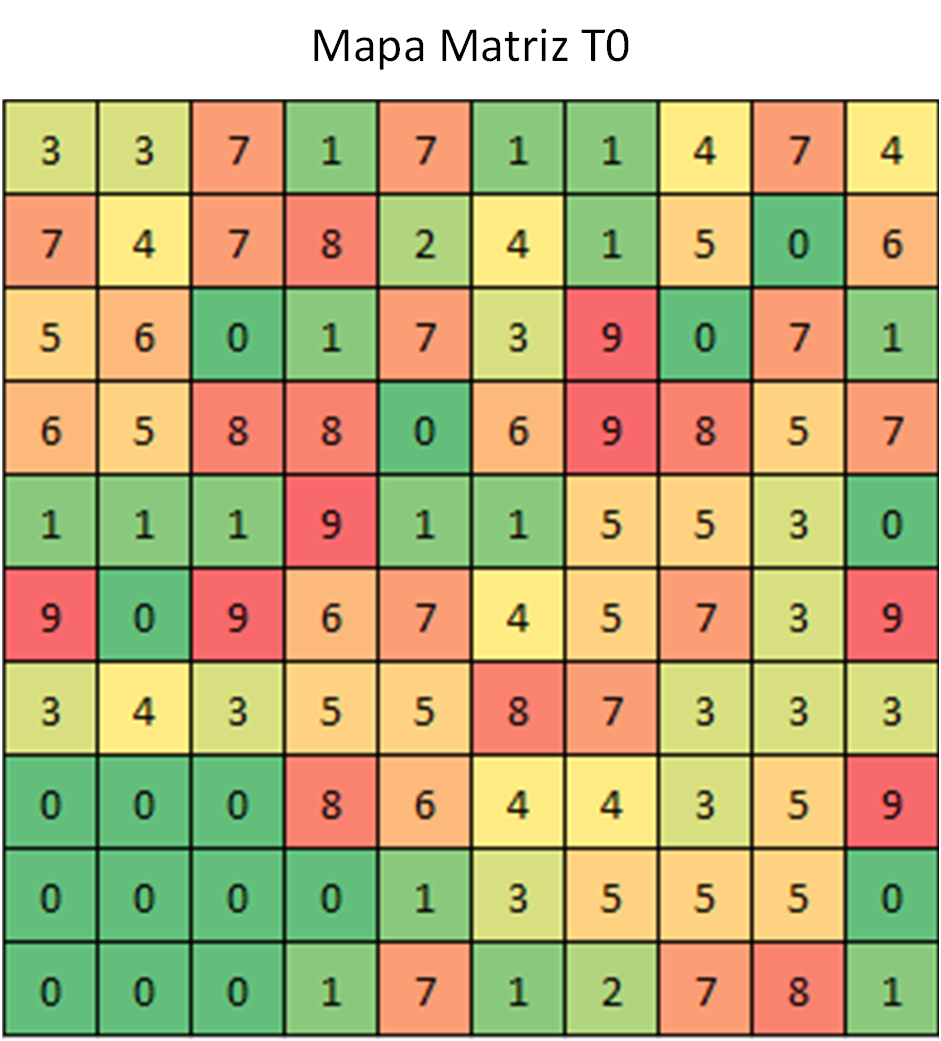
\includegraphics[scale=0.6]{Figuras/PonderationsExample-MatrixMap.png}
	\caption{Exemplo de ponderação - MapaMatriz T0.}
	\label{fig:MapaMatrizT0}
\end{figure}

Na Figura \ref{fig:OnePondertion} pode-se observar que foi escolhido apenas um fator de ponderação, o que fez com que a operação de convolução se torne completamente inútil, não sendo necessário seu cálculo, pois o fator aplicará como resultado do cálculo de apenas uma ponderação um crescimento homogêneo por quase todo o mapa, por exemplo, para um ponto qualquer \((x,y)\), este deve ser calculado na matriz de ponderação como:

\begin{equation}
\label{eq:ponderation1}
\begin{split}
Ponderação(x,y) = \sum_{i=0}^{PonderationCount} \left(\frac{Convolution(x,y) \cdot Fator[i]}{Convolution(x,y)}\right)
\end{split}
\end{equation}

Assim o ponto (0,0) seria:

\[Pond1(0,0) = \frac{Convolution(0,0) \cdot Fator1}{ Convolution(0,0)};\]
\[Pond1(0,0) = \frac{141 \cdot 0,5}{ 141 } = 0,5;\]


\begin{figure}[h]
	\centering	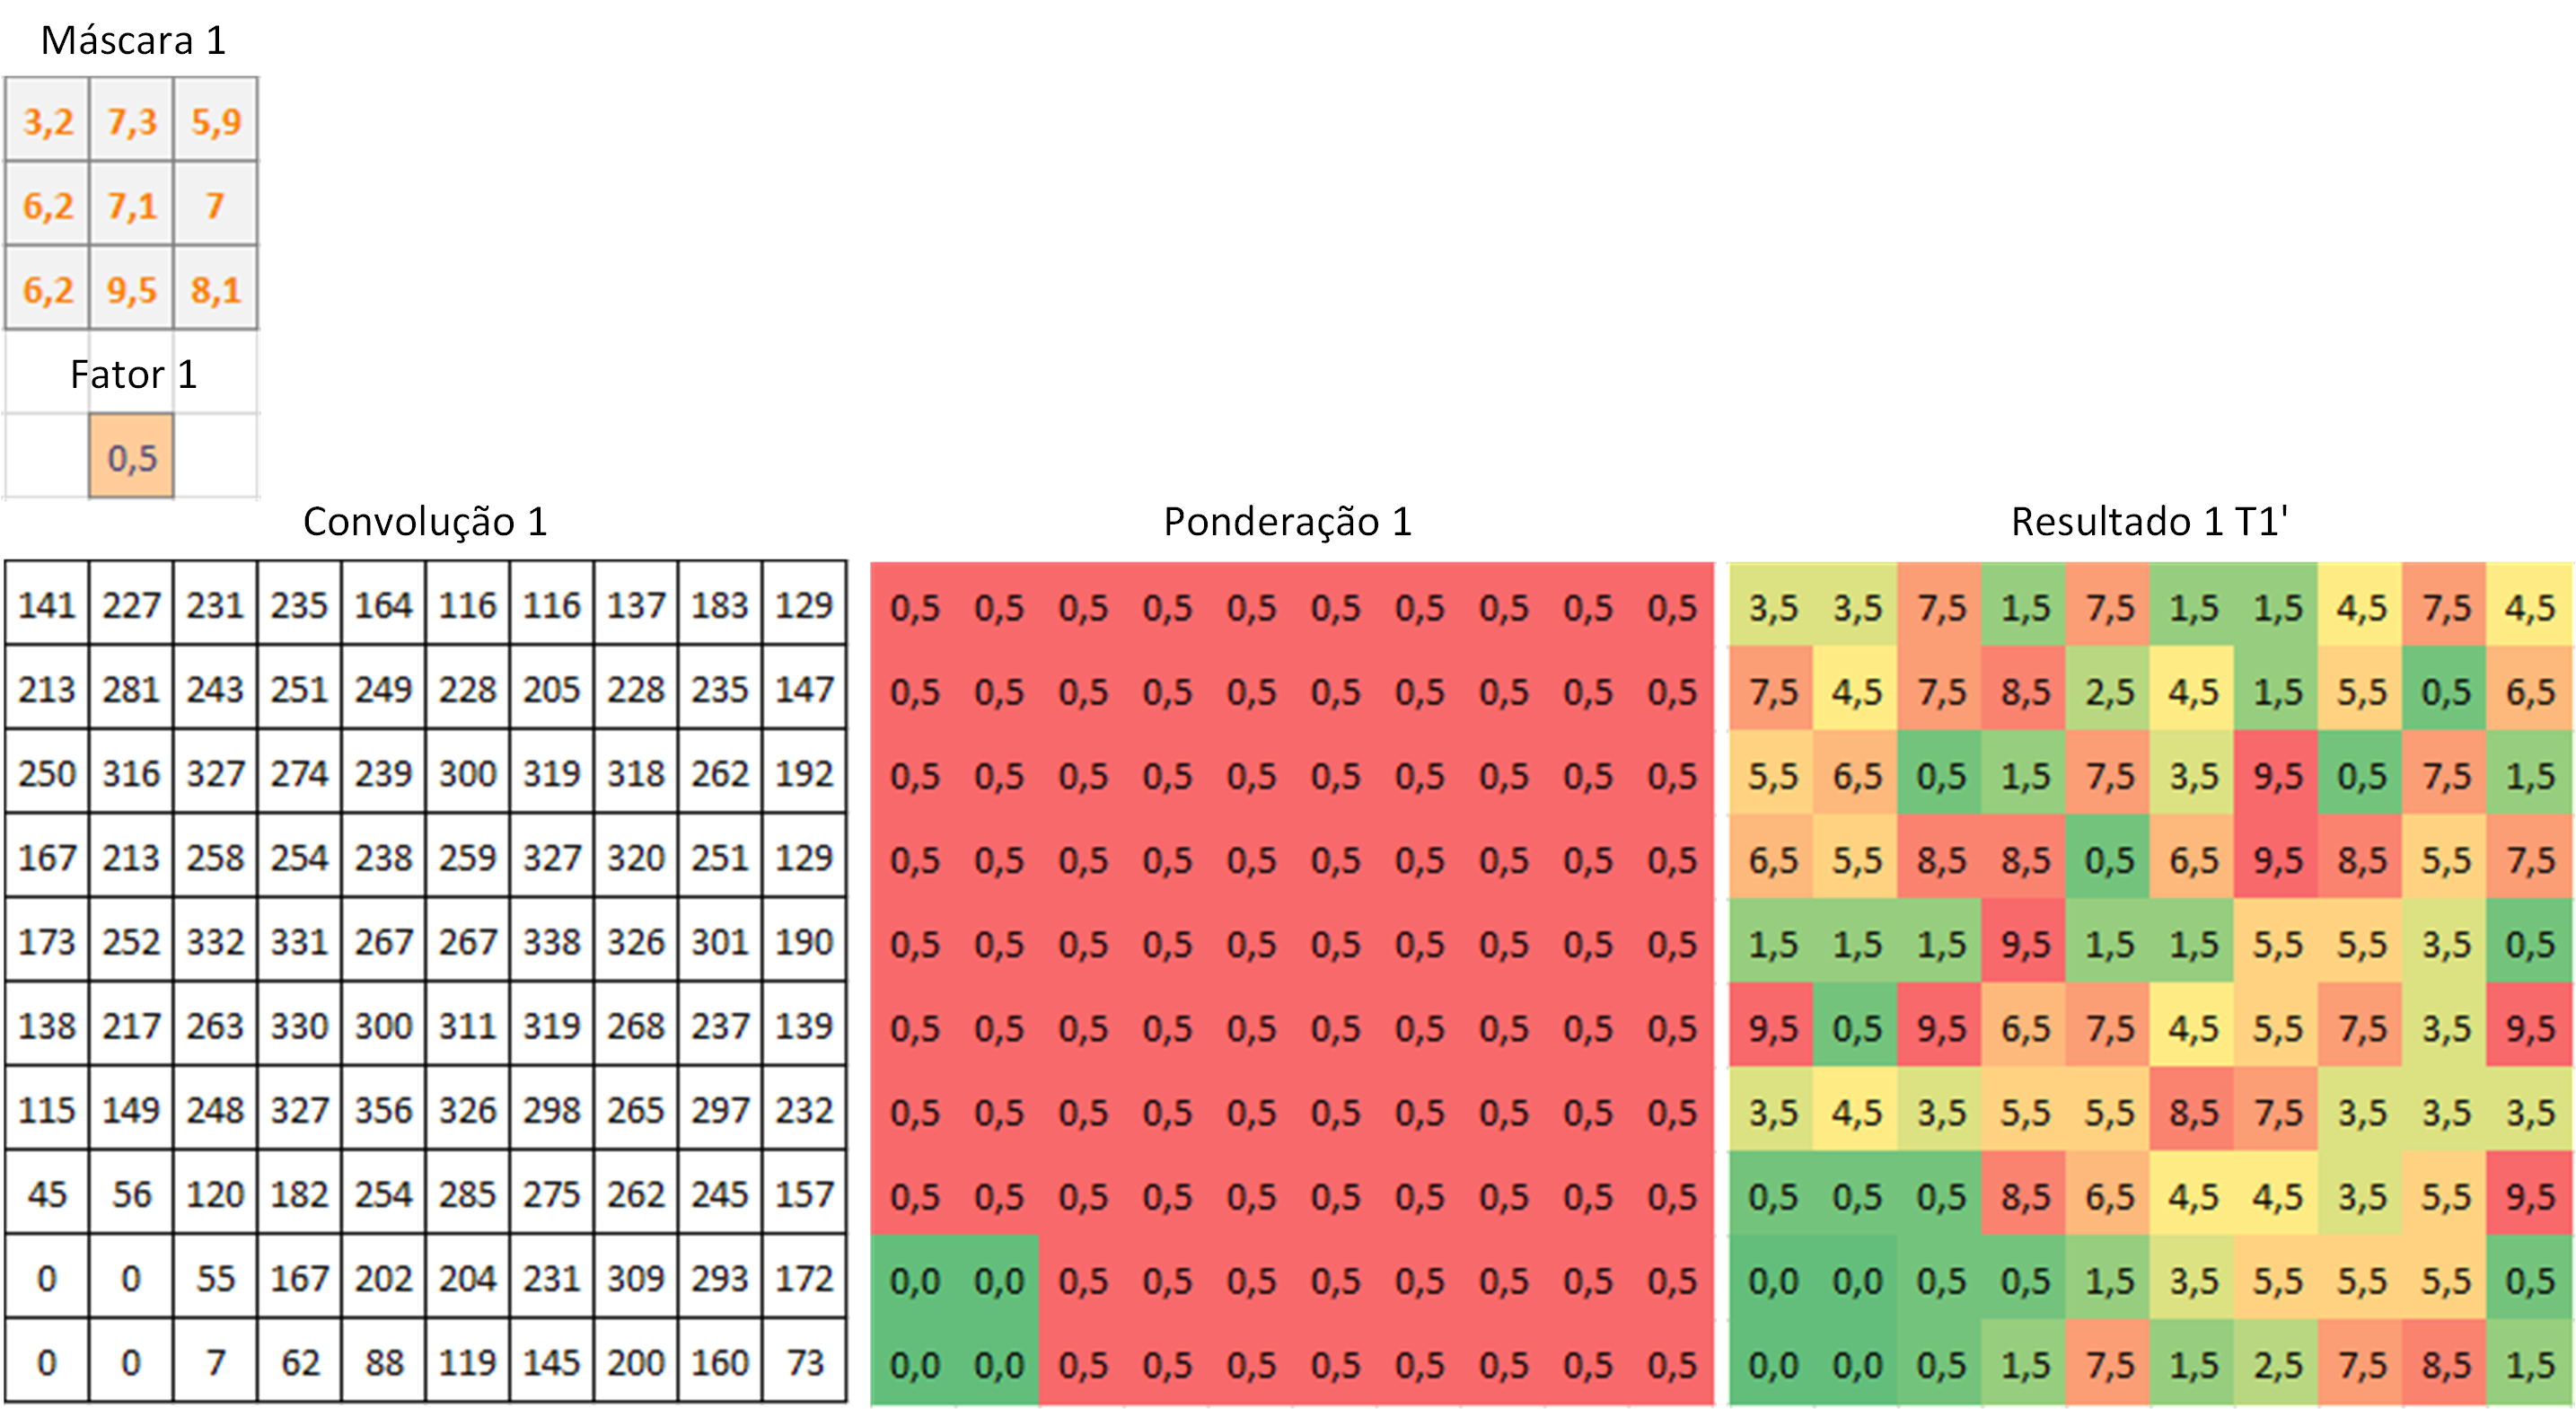
\includegraphics[scale=0.6]{Figuras/PonderationsExample-1Ponderation.png}
	\caption{Exemplo de ponderação - 1 ponderação}
	\label{fig:OnePondertion}
\end{figure}

Observe que se houver apenas uma ponderação o processo evolutivo tenderá ao crescimento médio da região durante os períodos, que neste caso levaria a uma previsão similar às apresentadas por técnicas estatísticas que usam a linha de tendência de crescimento aplicadas ponto a ponto, neste caso região por região. Ainda assim, este método demonstra um crescimento que expande ao longo dos períodos, pois no canto inferior esquerdo houve a expansão de 1 quadrícula sobre os valores que antes eram nulos. A matriz Resultado \emph{T1} é basicamente a soma ponto a ponto da matriz Ponderação 1 com o Mapa Matriz T0 (da Figura \ref{fig:MapaMatrizT0}).

Ao se adicionar mais um fator de ponderação, como mostra a Figura \ref{fig:TwoPondertion}, já é possível notar que o mapa de ponderação gerado não é mais homogêneo como o anterior, e que os cálculos de cada ponto do mapa de ponderações leva em consideração o valor de seus vizinhos. E ainda, o mapa \emph{Resultado 2} \emph{T1’} apresenta-se muito semelhante ao mapa anterior, crescendo não homogeneamente nesta região. A matriz \emph{Ponderação 2} segue o mesmo cálculo apresentado em \ref{eq:ponderation1}, usando as matrizes \emph{Convolução 1} (da Figura \ref{fig:OnePondertion}) e \emph{Convolução 2} (da Figura \ref{fig:TwoPondertion})

\begin{figure}[h]
	\centering	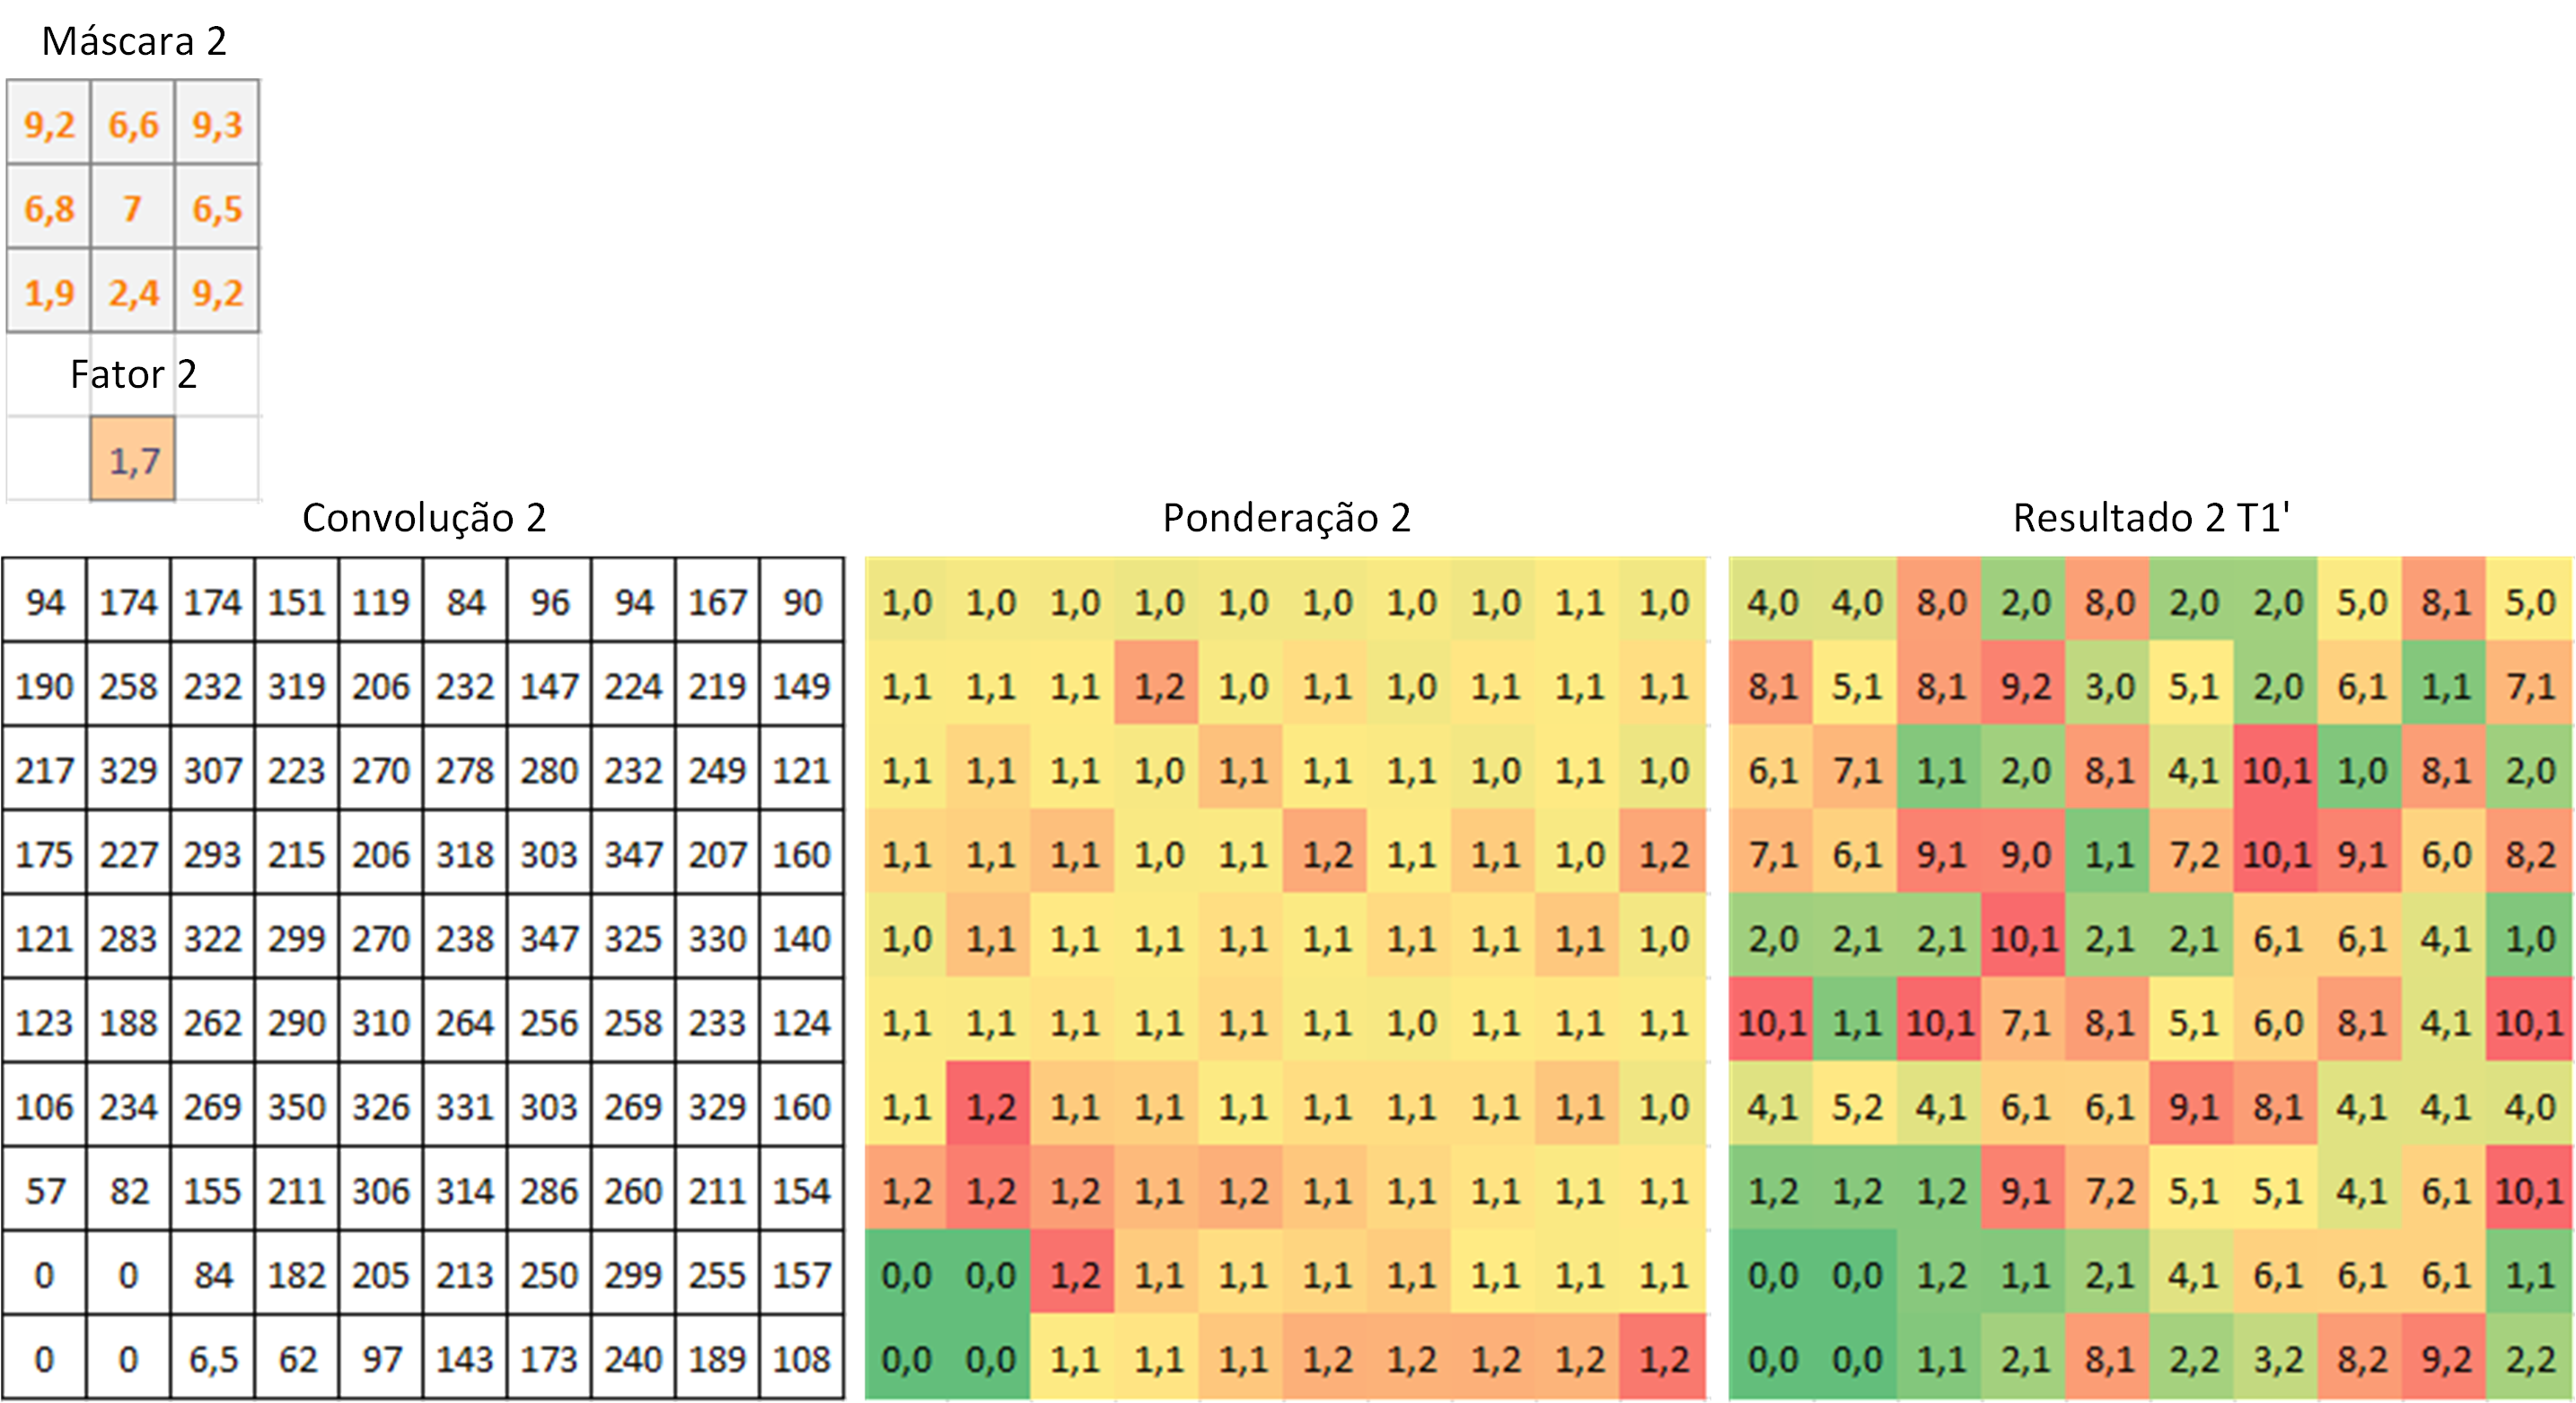
\includegraphics[scale=0.6]{Figuras/PonderationsExample-2Ponderations.png}
	\caption{Exemplo de ponderação - 2 ponderações}
	\label{fig:TwoPondertion}
\end{figure}

Por fim, a Figura \ref{fig:TreePondertion}, aumenta-se o número de ponderações para 3, o que consequentemente leva a 3 fatores de ponderação com a necessidade do cálculo de 3 matrizes de convolução e geração aleatória de 3 máscaras de convolução. Neste caso, observa-se que o fator apresenta um valor negativo, que decresce todo o crescimento do mapa mas mantém um padrão de crescimento muito similar ao anterior (apresentado pela Figura \ref{fig:TwoPondertion}). 

\begin{figure}[h]
	\centering	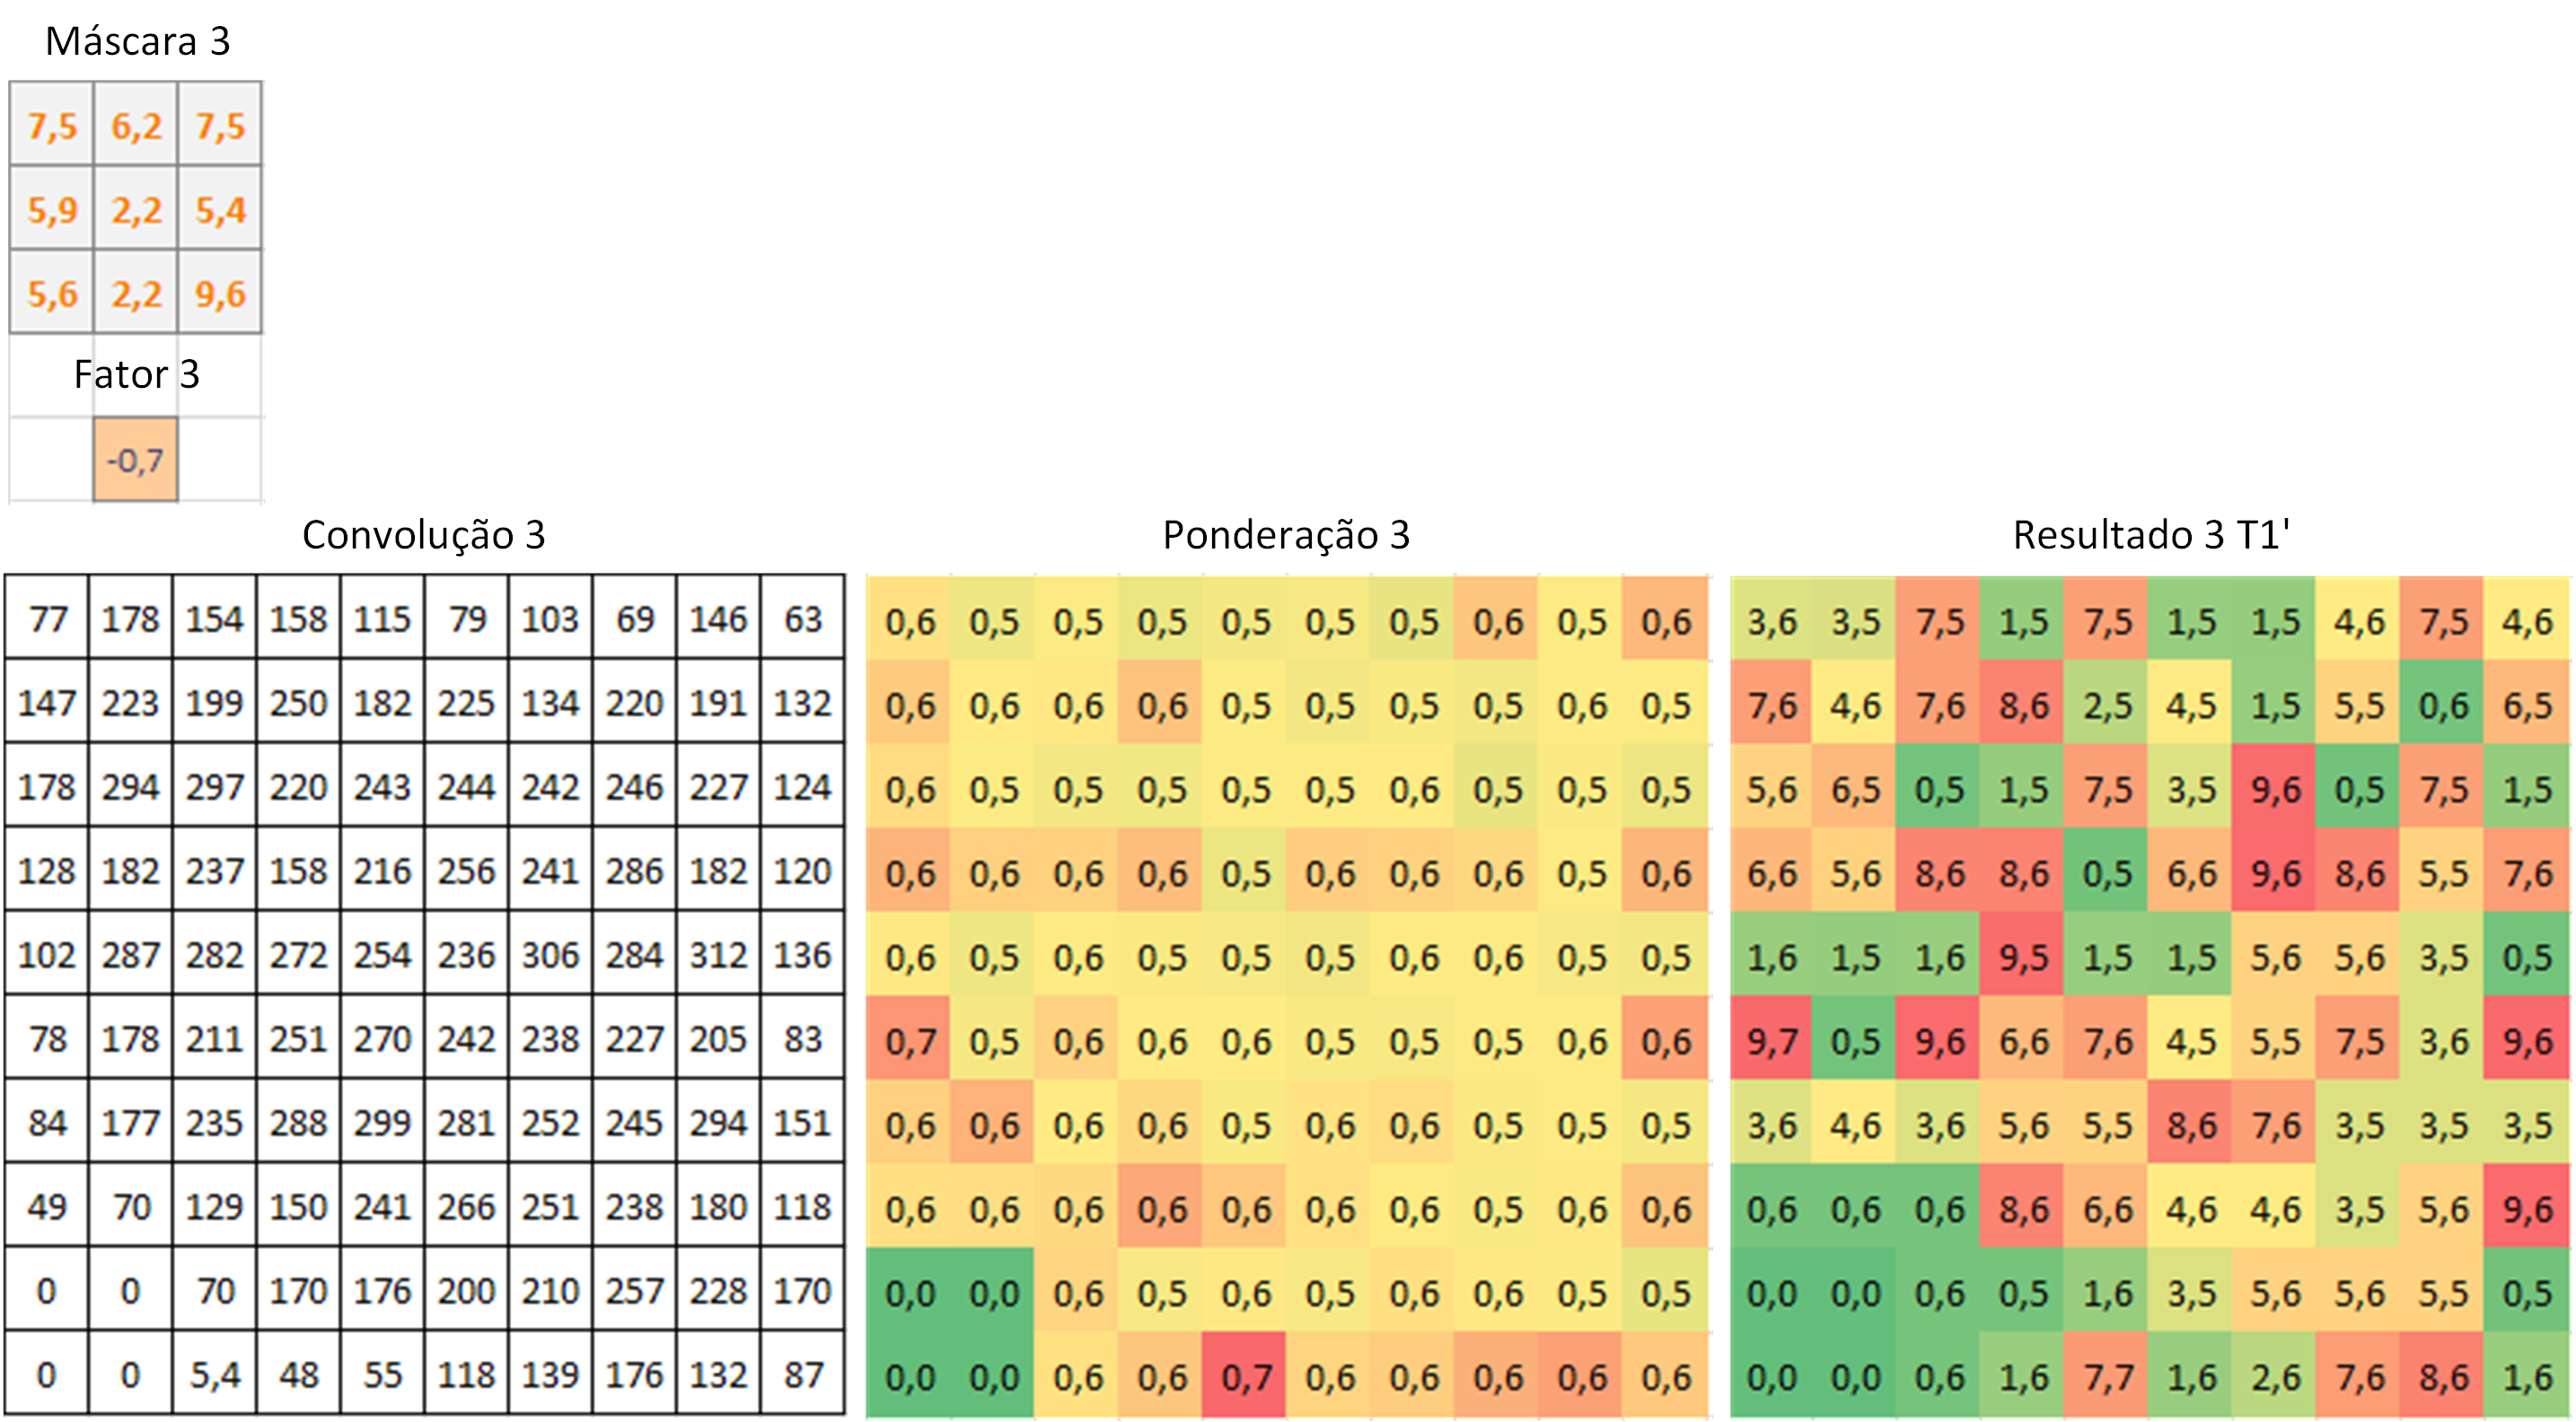
\includegraphics[scale=0.6]{Figuras/PonderationsExample-3Ponderations.png}
	\caption{Exemplo de ponderação - 3 ponderações}
	\label{fig:TreePondertion}
\end{figure}

Neste caso, com três ponderações, é possível notar que os valores dos fatores de ponderação geram valores para os pontos tal que estes serão diferentes porém com uma tendência à média dos fatores, e também são limitados na soma dos fatores. O que proporciona esta diferenciação entre os valores são as matrizes de convolução, que são usadas como ajuste, de modo que cada máscara gere uma matriz que releve uma ou mais características do mapa a ser ponderada, com o fator, neste caso, fazendo o papel de relevar ou não a característica em questão. 

Assim, é possível notar, que neste caso totalmente aleatório já existe uma tendência de crescimento geral, onde algumas regiões crescem mais que outras, de forma não homogênea, definida por características do mapa do período base, podendo assim, repetir-se tal processo para que tal tendência seja aplicada novamente sobre o mapa Resultado gerado, a fim de gerar uma previsão futura de um próximo período seguindo esta mesma tendência de crescimento. 

Espera-se então, que ao fim do processo evolutivo, realizado pelo ICA, ao aplicar esta técnica, que leva como parâmetros de previsão o conjunto de valores compostos por máscaras e fatores, seja possível gerar uma previsão tendenciosa, ou seja, que segue a curva de tendência de crescimento para a região, de forma não homogênea, ressaltando pontos de maior e menor crescimento dependentes de características adquiridas pelos ajustes dos valores, principalmente dos valores das máscaras de convolução, e por fim de forma apresentável bidimensionalmente, de modo que tal região venha compor o mapa final. 








\section{Aplicando o ICA}
\label{Aplicando o ICA}

Para que o ICA seja inicializado apropriadamente, de forma a gerar soluções que possam ser usadas para prever a densidade espacial de carga períodos a frente, é necessário que se modele o problema como foi feito nos problemas G1 e G2, descritos neste capítulo na seção \ref{Exemplos de aplicação do ICA genérico}. Assim, é necessário que sejam definidos, a função de avaliação, o que cada dimensão representará durante o processo evolutivo, e consequentemente a quantidade de dimensões. Deve-se também antes de iniciar o processo evolutivo definir quais são os limites de cada dimensão definida.

A modelagem do problema da previsão da densidade espacial de carga para otimização pelo ICA, se resume em uma implementação da interface \emph{IFitness}, de forma que tal implementação seja capaz de evoluir os valores, ou atributos, dos indivíduos, a fim de que a melhor solução possa ser aplicada na base de dados para se gerar previsões. Observa-se que para obter uma previsão sobre os dados é necessário utilizar o ICA para evoluir os indivíduos até um período antes do que se deseja gerar a previsão (sobre dados históricos, em forma dos mapas matrizes particionados), e então utilizar os indivíduos evoluídos junto deste último período, passando-os pela função de previsão usada durante a avaliação, a fim de gerar uma previsão para o próximo período. Para fazer a previsão de mais de um período à frente, basta utilizar o resultado obtido da previsão do período anterior e executar novamente a função de previsão, que irá gerar desta vez uma previsão sobre um período já previsto, acumulando assim o erro de previsão inicial (base inicial \(\Rightarrow\) previsão1) e o erro de previsão atual (previsão1 \(\Rightarrow\) previsão2). Quanto mais períodos forem previstos mais erro acumulado será gerado nas previsões futuras.

A técnica utilizada para fazer com que os elementos do ICA possam evoluir, e fornecer as melhores soluções, tal que quando aplicadas sobre os dados para períodos futuros, devem fornecer previsões espaciais da região selecionada. Assim  entende-se que a função avaliação deve ser dependente do tempo, e este tempo, será definido como o número de períodos selecionados para o problema, por serem espaçados igualmente. Porém a intenção não é fazer uma previsão de crescimento para cada quadrícula presente no mapa, uma vez que a intenção é buscar também a influência que os vizinhos aplicam sobre a quadrícula, elaborando assim, uma técnica que leva em consideração uma quantidade de quadrículas, de modo que se defina um padrão de crescimento médio, relativo tanto ao crescimento do ponto quanto à evolução da forma da região em questão. Tendo assim, no final, um mapa que forme regiões de maior possibilidade de ocorrência de aumento de densidade para os períodos futuros.

Tem-se que o mapa é representado como uma imagem através dos mapas matrizes para cada período, então foi elaborada uma técnica  semelhante a técnica apresentada no problema G2 na seção \ref{Exemplos de aplicação do ICA genérico}, a qual buscará pela melhor solução, de forma que se encontrem os melhores filtros ou matrizes de convolução, porém, neste caso,  ponderados de acordo com suas relevâncias, tal que estes filtros quando aplicados na matriz de um período \(t0\) opere gerando uma nova matriz \(t1’\), que seja mais semelhante possível à matriz do período \(t1\), e quando aplicada à matriz do período \(t1\), opere gerando uma nova matriz \(t2’\), que seja mais semelhante possível ao período \(t2\), e assim por diante.

Um grande problema, não apenas para este tipo de solução, mas para todas as técnicas de previsão, é a previsão futura que leva em consideração muitos períodos a frente, e que utilizam-se dos períodos anteriores para prever o novo período, é  referente ao grande acúmulo de erro durante a previsão para estes períodos futuros mais distantes da origem.Então sabe-se que a previsão tem um bom resultado para os períodos iniciais e acumulará mais erro para os períodos futuros. Entretanto, insere-se um fator na avaliação a fim de fazer com que as matrizes ou filtros de convolução, durante a evolução, levem em consideração a taxa de crescimento média daquela região, o que ajuda a diminuir um pouco deste erro, e faz com que a solução tenha uma tendência para o crescimento médio desta região.


\subsection{Modelando os países avaliação}
\label{Avaliação dos países}

A avaliação do problema deve fornecer indivíduos capazes de efetuar uma previsão de densidade espacial, sobre a região apresentada, para um ou mais períodos à frente, a partir de um conjunto de mapas matrizes e os índices de crescimento absoluto durante os períodos. Assim, a avaliação de cada indivíduo irá ser resumida nas etapas:

\begin{itemize}
\item Tradução do vetor de atributos dos países;
\item Processamento dos mapas de previsão; 
\item Cálculo parcial do erro;
\item Avaliação dos erros e atribuição do custo;
\end{itemize}

A tradução do vetor de atributos basicamente transforma o vetor de atributos de um dado país, em estruturas mais práticas para o processamento, tal que o acesso ao vetor de atributos seja minimizada e o gerenciamento dos elementos sejam simplificados, gerando assim, um vetor de valores unitários, contendo os valores de ponderação, e um vetor de filtros, ou máscaras, do mesmo tamanho do vetor anterior, contendo matrizes que representam os filtros que serão usados para a convolução.   

O processamento dos mapas de previsão é a parte principal da avaliação, e é responsável por reproduzir o processo de previsão sobre os mapas matrizes existentes, o qual será usado para efetuar a previsão real, assim que o ICA terminar a competição imperialista, fornecendo o melhor país como solução. Esta etapa então, itera por todos os mapas matrizes, com exceção do último, utilizando as máscaras de convolução, transformadas do vetor de atributos do país, para gerar mapas que sejam o resultado da convolução entre o mapa matriz do período em questão com as matrizes de convolução provindas de cada ponderação, gerando assim vários mapas matrizes. A partir destes mapas resultantes, gera-se então um mapa ponderado, sendo este a ponderação dos mapas resultantes da convolução, onde os fatores de ponderação são os contidos no vetor de valores unitários de ponderações, traduzido dos atributos dos países. Assim, com este mapa final ponderado dos diversos mapas de convolução, gera-se um mapa final que é o resultado da soma do mapa deste período com o mapa ponderado, sendo este mapa final o mapa previsto para o período seguinte, \(t_1’\), sendo \(t_0\) o período atual. 

Antes mesmo de sair da iteração principal, pelos mapas matrizes, calcula-se a diferença entre o mapa de previsão e o mapa real do próximo período, e tais diferenças são usadas então, para gerar os erros produzidos em cada iteração. O cálculo dos erros leva em conta ainda o crescimento absoluto que cada período tem para com o seu próximo, então, se a diferença pode ser calculada como mostra expressão \ref{eq:forecastdif}:

\begin{equation}
\label{eq:forecastdif}
dif = ABS( Mapa[t_1] - Mapa[t_1’] ).
\end{equation}
	
Para se calcular o erro total gerado durante este período, levando em consideração o mapa de previsão e o crescimento em relação ao período de forma igualitária, fazendo-se a multiplicação da diferença \(dif\) por \(0.5\), e então soma-se com o valor de crescimento absoluto entre os períodos \(t_x\) e \(t_{x+1}\), que também é multiplicado por \(0.5\). Sendo assim, este valor final de erro para o dado período \(t_x\), ou iteração atual,é armazenado em um vetor de erros \(Errors\) que armazenará todos os erros gerados a durante cada iteração entre os períodos em que se fará a previsão, como mostra a expressão \ref{eq:forecasVectortError}:

\begin{equation}
\label{eq:forecasVectortError}
	Errors[t_x] = dif \cdot 0.5 + CrescimentoAbsoluto[t_x \Rightarrow t_{x+1}] \cdot 0.5.
\end{equation}

A utilização do crescimento absoluto na função de avaliação poderia ser removida, que o resultado seria algo muito parecido se não o mesmo, porém este fator é inserido para que o processo evolutivo chegue mais rapidamente ao resultado esperado, de modo que tal influência acelere e refine o resultado final do país. Por fim, durante a última e mais simples etapa, somam-se todos os erros e atribui ao valor de custo do país em questão, finalizando assim a avaliação de um indivíduo. 

Este processo de avaliação faz com que o país, ao longo das eras tenha seus atributos convergindo para a melhor solução, operando a convolução e ponderando os mapas matrizes tal que o erro gerado pelo mapa de previsão seja o mais próximo do mapa real e também, tal que seu crescimento seja predito de acordo com o crescimento entre os períodos reais. 

A ponderação entre os mapas de convolução, ao invés de apenas usar uma operação de convolução diretamente, sem ponderação, é necessária para que o mapa final resulte em uma previsão mais exata. Pois entende-se que ao tentar buscar uma matriz de convolução entre duas imagens, as quais uma é o resultado da passagem da matriz de convolução sobre a outra, como descrito no problema G2, é um problema diferente do objetivo do trabalho, o qual é mais simples, apesar da complexidade da solução, por se saber que existe, de fato, um filtro ou matriz de convolução que leva uma imagem ser transformada em outra, quando operada a convolução. Já o problema proposto, a diferença entre um período e outro não é apenas a busca por uma matriz de convolução, mas sim a previsão, que para isto, são usadas matrizes de convolução com seus resultados ponderados, onde cada uma destas matrizes de convolução agrega uma ou mais características da região durante um dado período, que são relevadas pelo fator de ponderação. Observa-se que o problema proposto ainda utiliza as mesmas matrizes de convolução para operar por todos os períodos, então se houverem várias características que possam vir a ser identificadas durante todos os períodos, as matrizes terão mais liberdade de adaptação, sendo que tais características podem variar entre as máscaras de convolução e ser ponderadas de acordo com suas relevâncias. Observa-se ainda, que a intenção não é obter o resultado exato, mas sim uma matriz que gere um mapa semelhante que possa ser usado para previsão futura das regiões.

A Figura \ref{fig:ForecastEvalPart0}  ilustra uma situação de avaliação para cinco períodos, \(t0\), \(t1\), \(t2\), \(t3\) e \(t4\), tais que máscaras de convolução, \(Masks 1,2,...,n\), geram mapas matrizes, \(t1’(1,2,...,n)\), \(t2’(1,2,...,n)\), \(t3’(1,2,...,n)\) e \(t4’(1,2,...,n)\), que são ponderados para gerar mapas de previsão, \(T1’\), \(T2’\), \(T3’\) e \(T4’\).

\begin{figure}[h]
	\centering	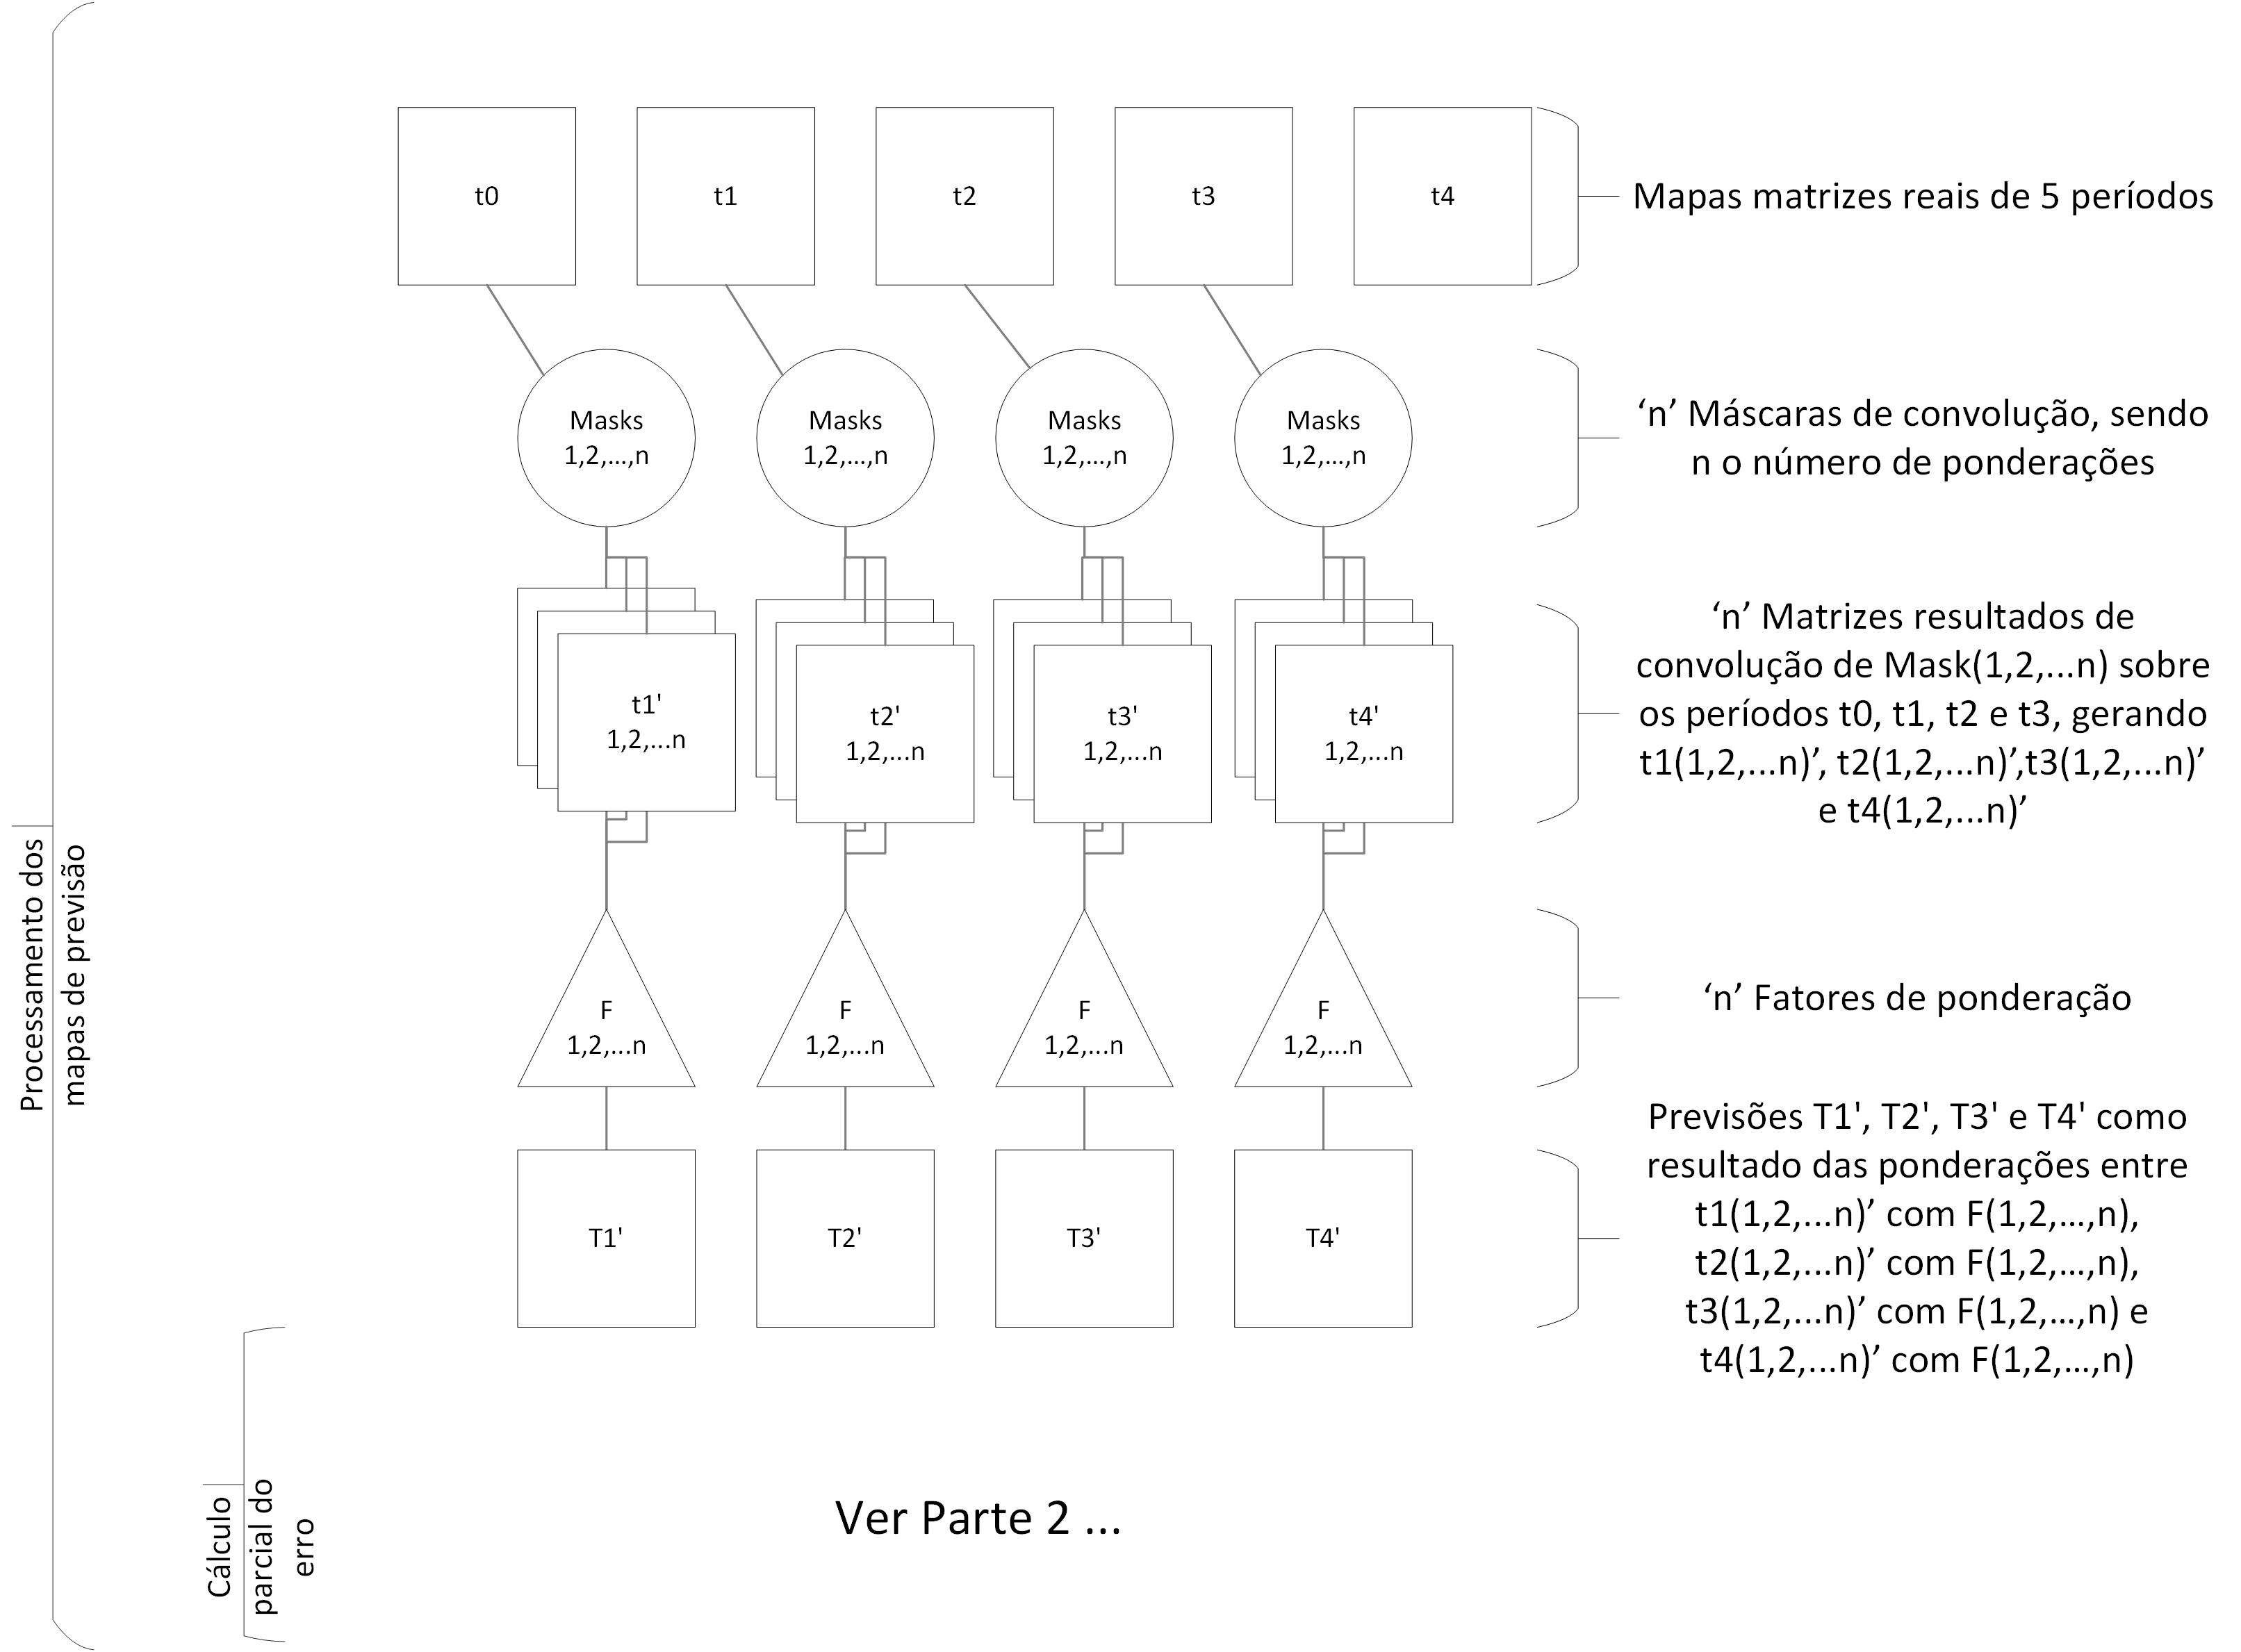
\includegraphics[scale=0.55]{Figuras/Ilustrations-ForecastEvalPart0.png}
	\caption{Processamento dos mapas de previsão parte 1.}
	\label{fig:ForecastEvalPart0}
\end{figure}

Já a Figura \ref{fig:ForecastEvalPart1}  mostra como os cálculos parciais são executados, sendo que faz-se o uso dos mapas matrizes de previsão e dos mapas matrizes reais tal que se tenha no final, armazenados no vetor \emph{resultValues}, os erros gerados de modo que este vetor possa ser usado para que se atribua o custo do país na próxima etapa de avaliação dos erros e atribuição do custo.

\begin{figure}[h]
	\centering	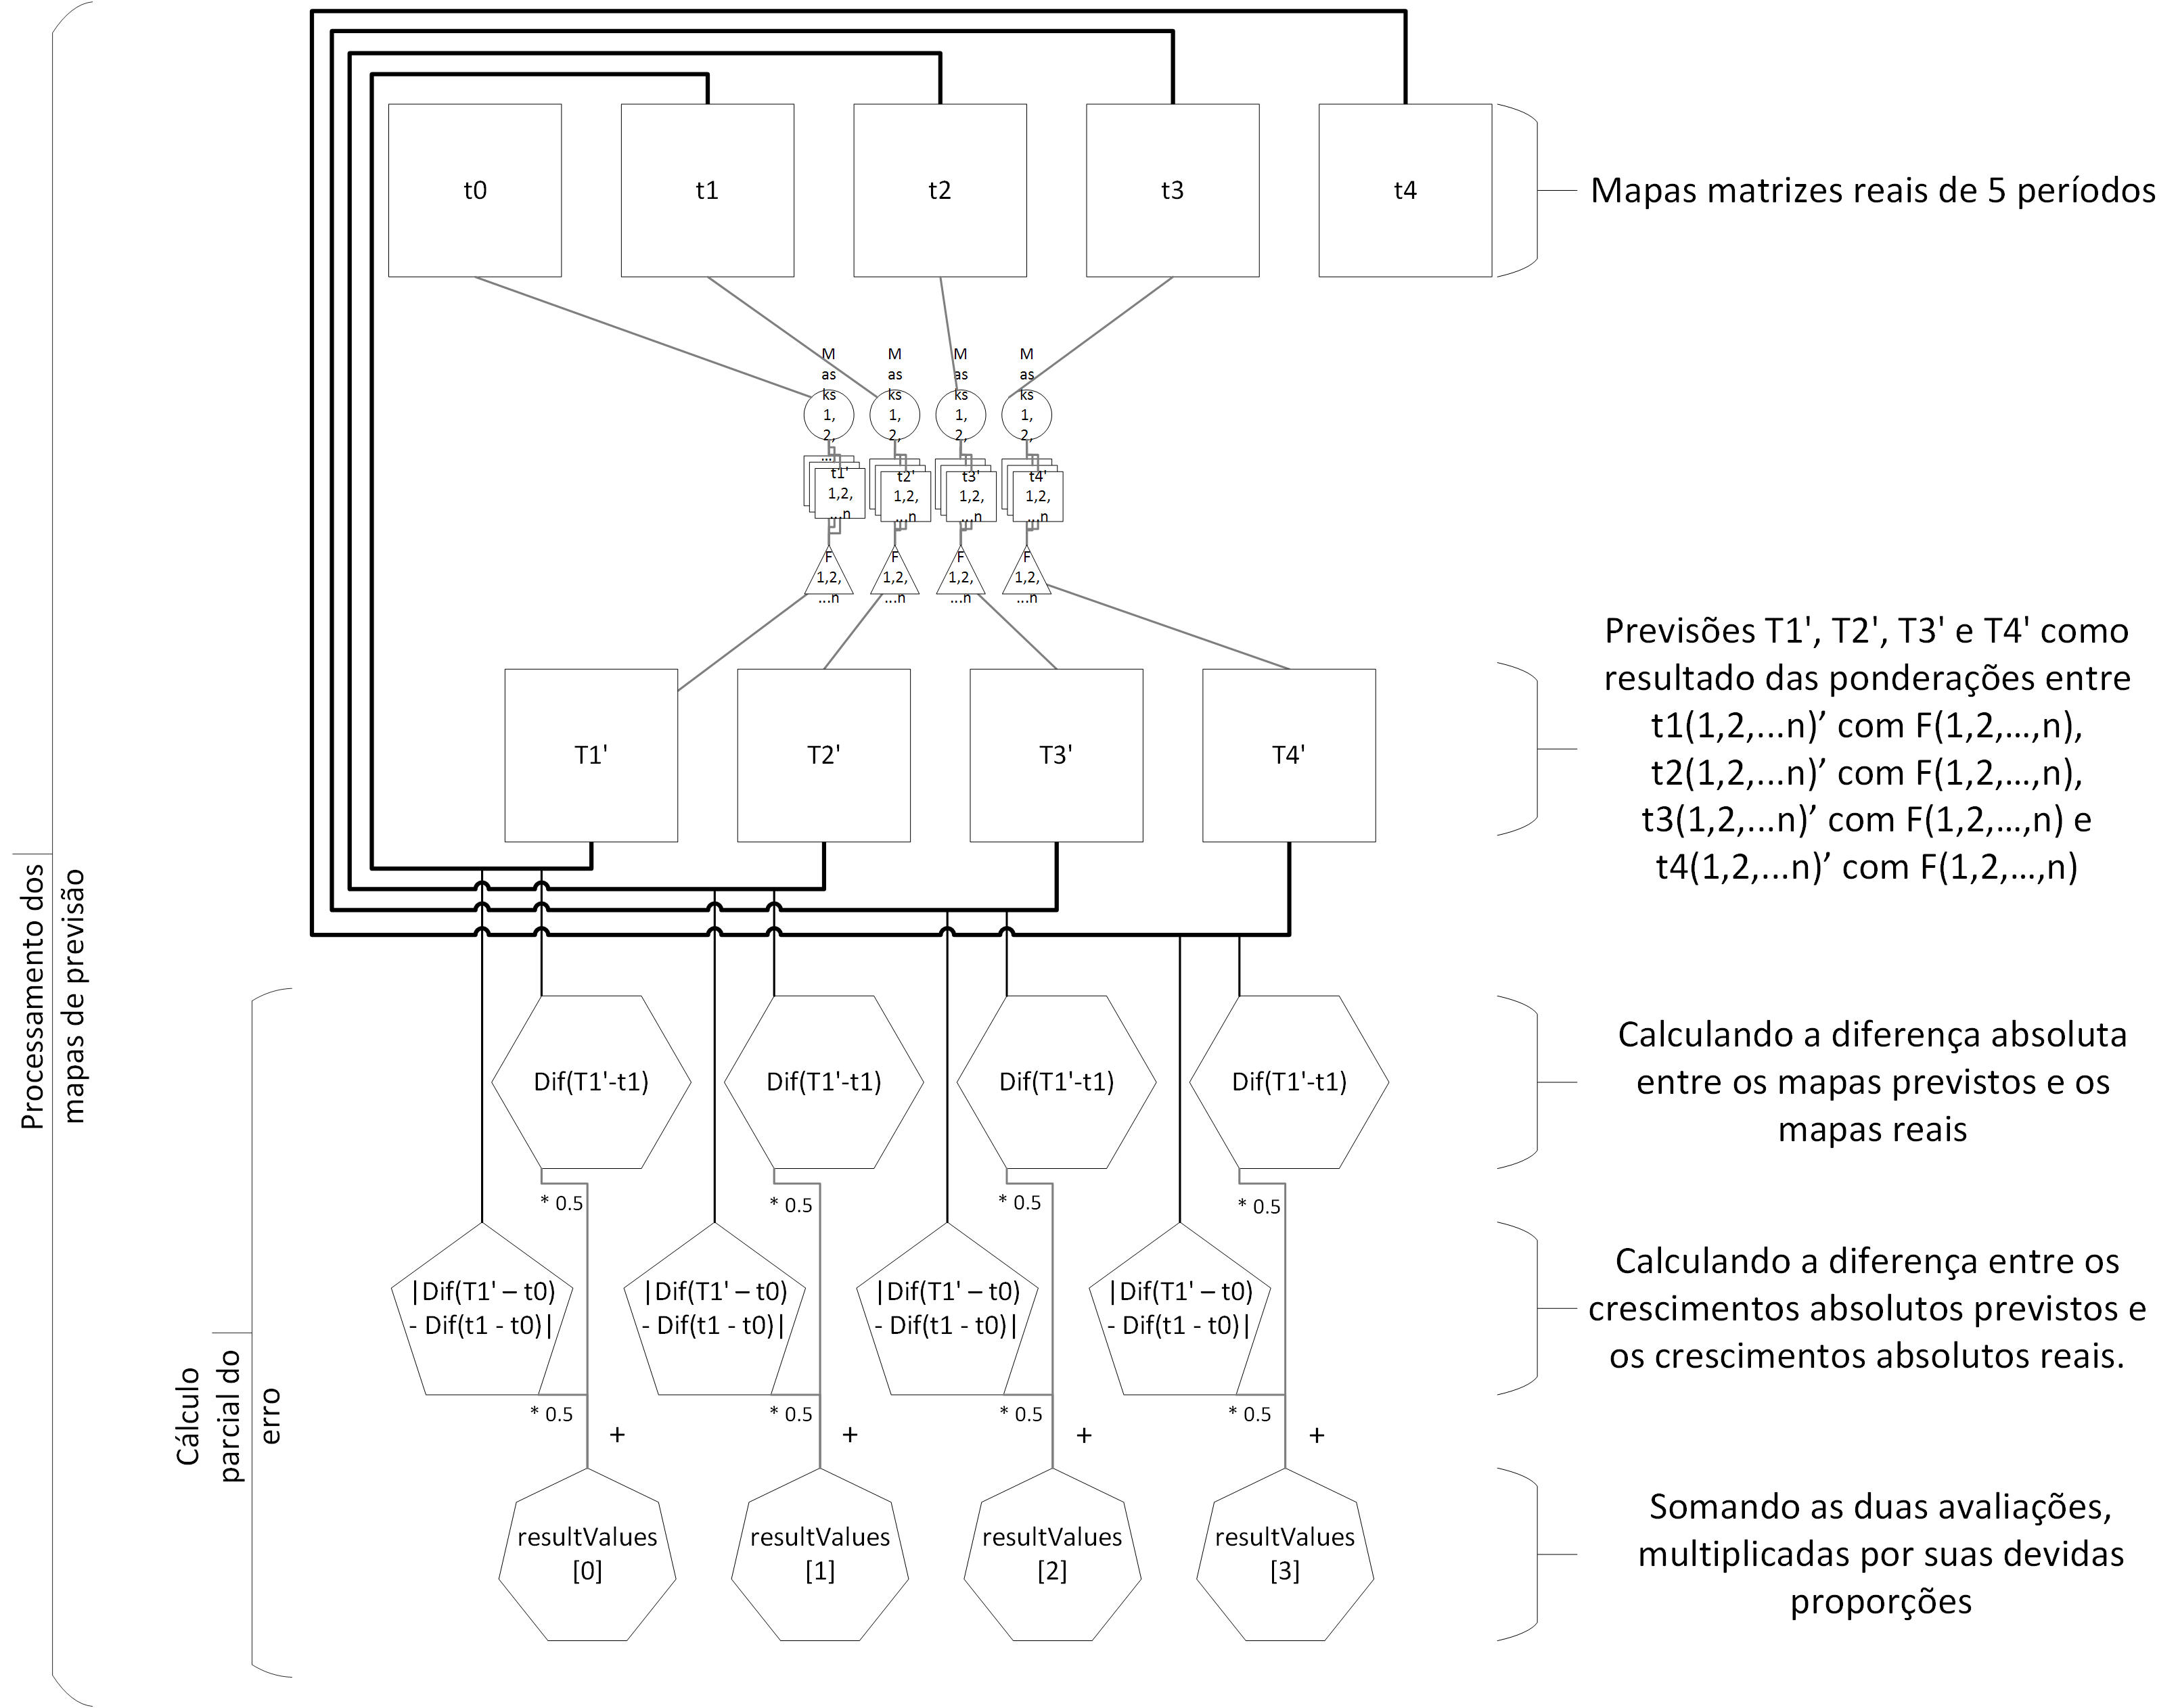
\includegraphics[scale=0.55]{Figuras/Ilustrations-ForecastEvalPart1.png}
	\caption{Processamento dos mapas de previsão parte 2.}
	\label{fig:ForecastEvalPart1}
\end{figure}

Assim, resumidamente o que ocorre no processamento dos mapas de previsão durante a evolução, é a utilização de todos os períodos para uma forma de treinamento dos países competidores no ICA tal que estes sejam capazes, quando aplicados a um dado período, de produzirem um período à frente do período utilizado, como mostra a expressão:

\begin{equation}
\label{eq:forecastError}
Mapa(t_1’) = F(Mapa(t_0), País)
\end{equation}

De modo que durante as próximas etapas, sejam calculados os erros, comparando o mapa de previsão gerado em \(Mapa(t_1’)\) com o mapa real do período \(Mapa(t_1)\), tanto em semelhança quanto em crescimento absoluto. Atribuindo assim este erro como sendo o custo do país, a fim de se obter um país, para que o ICA, então, retome seu processo evolutivo, que decidirá através das operações já mencionadas se este país possui atributos melhores que os demais, terminando assim a etapa de avaliação dos países, que ocorre muitas vezes até que se chegue em um resultado otimizado, o qual satisfaça as condições de parada.




\subsection{A função de avaliação}
\label{A função de avaliação}

A primeira etapa da implementação da função de avaliação, que é definida pelo problema em questão, para ser processado pelo ICA, é a definição da interface \emph{IFitness} e consequente implementação de seus métodos e propriedades em uma classe chamada \emph{PonderationFullConvolutionFitness}. A implementação desta interface, independente da implementação dos métodos ou propriedades, divide-se nas partes: 
\begin{itemize}
\item Definição de constantes e inicialização das constantes;
\item Definição do método de inicialização dos países;
\item Definição da função de avaliação e
Teste.
\end{itemize}

Começando então pela definição dos valores constantes e suas inicializações, para este problema é interessante manter uma cópia da lista de mapas matrizes, denominada \emph{MapsList}, em cache, de modo que esta lista possa ser acessada por múltiplas tarefas em paralelo (provindo de chamadas feitas paralelamente pelo ICA), evitando que haja escrita, pois o modelo utilizado para representar esta lista é seguro e não obstrutivo (\emph{Thread Safe}) apenas para leitura de dados da lista. Outros dois valores constantes que definem o vetor de atributos do país são:
\begin{itemize}
\item \emph{PonderationCount}, que define o número de ponderações e consequentemente quantas matrizes de convolução existirão;
\item \emph{Order}, que define qual será a ordem das matrizes de convolução. 
\item \emph{absoluteGrowths}, que define o crescimento absoluto entre os mapas matrizes período a período, sendo este valor calculado assim que se entra com os mapas matrizes na lista de mapas \emph{MapsList}.
\item \emph{maskCount}, que representa a quantidade de valores presente em cada máscara, utilizado para a definição do número de dimensões e durante a tradução da lista de atributos. 
\end{itemize}

Observe que estes dois últimos elementos poderiam não existir, porém, para que possa se otimizar a função de avaliação, que pode ser chamada milhares de vezes, calculam-se todos estes elementos independentes, evitando cálculos desnecessários durante as chamadas de avaliação.

O método de inicialização dos países é bem simples, uma vez que não insere dados de entrada nos atributos dos países e o problema não exigiu alteração das funcionalidades básicas do país. Assim, a inicialização dos países se resume na criação de uma lista de países do tamanho \emph{Dimensions}, que gera \emph{nPopulation} países com atributos uniformemente aleatórios, onde cada dimensão está limitada entre \emph{minBounds} e \emph{maxBounds}. Os valores \emph{nPopulation}, \emph{minBounds} e \emph{maxBounds} são parâmetros de entrada da função recebidos diretamente do ICA, os quais podem ser configurados antes de se chamar o método \emph{Run()} do ICA que evolui os países. Já o valor de \emph{Dimensions} é um cálculo que utiliza os valores definidos anteriormente e é definido a seguir,  em \ref{Atributos dos Países}, mostrando o que cada atributo presente nos países representa no problema e como eles são traduzidos para serem utilizados pela função de avaliação.





\subsubsection{Atributos dos Países}
\label{Atributos dos Países}

A partir da ideia gerada durante a modelagem da função de avaliação, definiu-se como deve ser modelado um país para que o ICA processe este problema e quais são os componentes do vetor de atributos a serem evoluídos durante a competição. Então como será feita uma ponderação de matrizes de convolução, em \emph{PonderationCount}, tem-se quantas ponderações devem ser feitas, em \emph{Order}, qual a ordem das matrizes de convolução. Assim, o número de atributos total que os países do ICA terão, definido em \emph{Dimensions}, na implementação do objeto que contém a função de avaliação, pode ser descrito como apresentado na expressão \ref{eq:forecastDimensions}: 
	
\begin{equation}
\label{eq:forecastDimensions}
\begin{split}
Dimensions = PonderationCount \cdot (maskCount + 1), 
\\\text{Onde}
\\maskCount = order \cdot order.
\end{split}
\end{equation}

A definição do valor de dimensões dos países é obrigatória e ocorre durante a inicialização do objeto que implementa a função de  avaliação (ou implementação da interface \emph{IFitness}), e faz parte da modelagem do problema. Note que não se define diretamente o valor de dimensões no país, mas sim na função de avaliação, para  que a solução fique genérica e dependa apenas da implementação da função de aptidão como demonstrado neste capítulo em \ref{ICA Orientado a Objetos}, e ainda, não se insere um valor fixo, mas sim na expressão \ref{eq:forecastDimensions} de modo que o número de dimensões ainda varie de acordo com os valores de número de ponderações e ordem da máscara de convolução.

Cada país usa a implementação padrão da classe \emph{Country} do ICA, sem nenhuma alteração, assim, todo indivíduo terá uma distribuição uniforme quando gerar os números aleatórios para seus atributos, tanto em sua inicialização quanto em chamadas que sorteiam estes atributos do indivíduo durante a evolução, causadas pela operação de revolução colonial.

A Figura \ref{fig:VetorAtributosForecast-Ingles} ilustra como os valores são dispostos no vetor de atributos do país. Observe que primeiro vem o valor de ponderação e em seguida vem os valores da máscara de convolução, formando um bloco. O número de blocos é dependente da quantidade de ponderações que se deseja gerar para um mapa, e o tamanho de cada bloco depende da ordem da matriz de convolução.

\begin{figure}[h]
	\centering	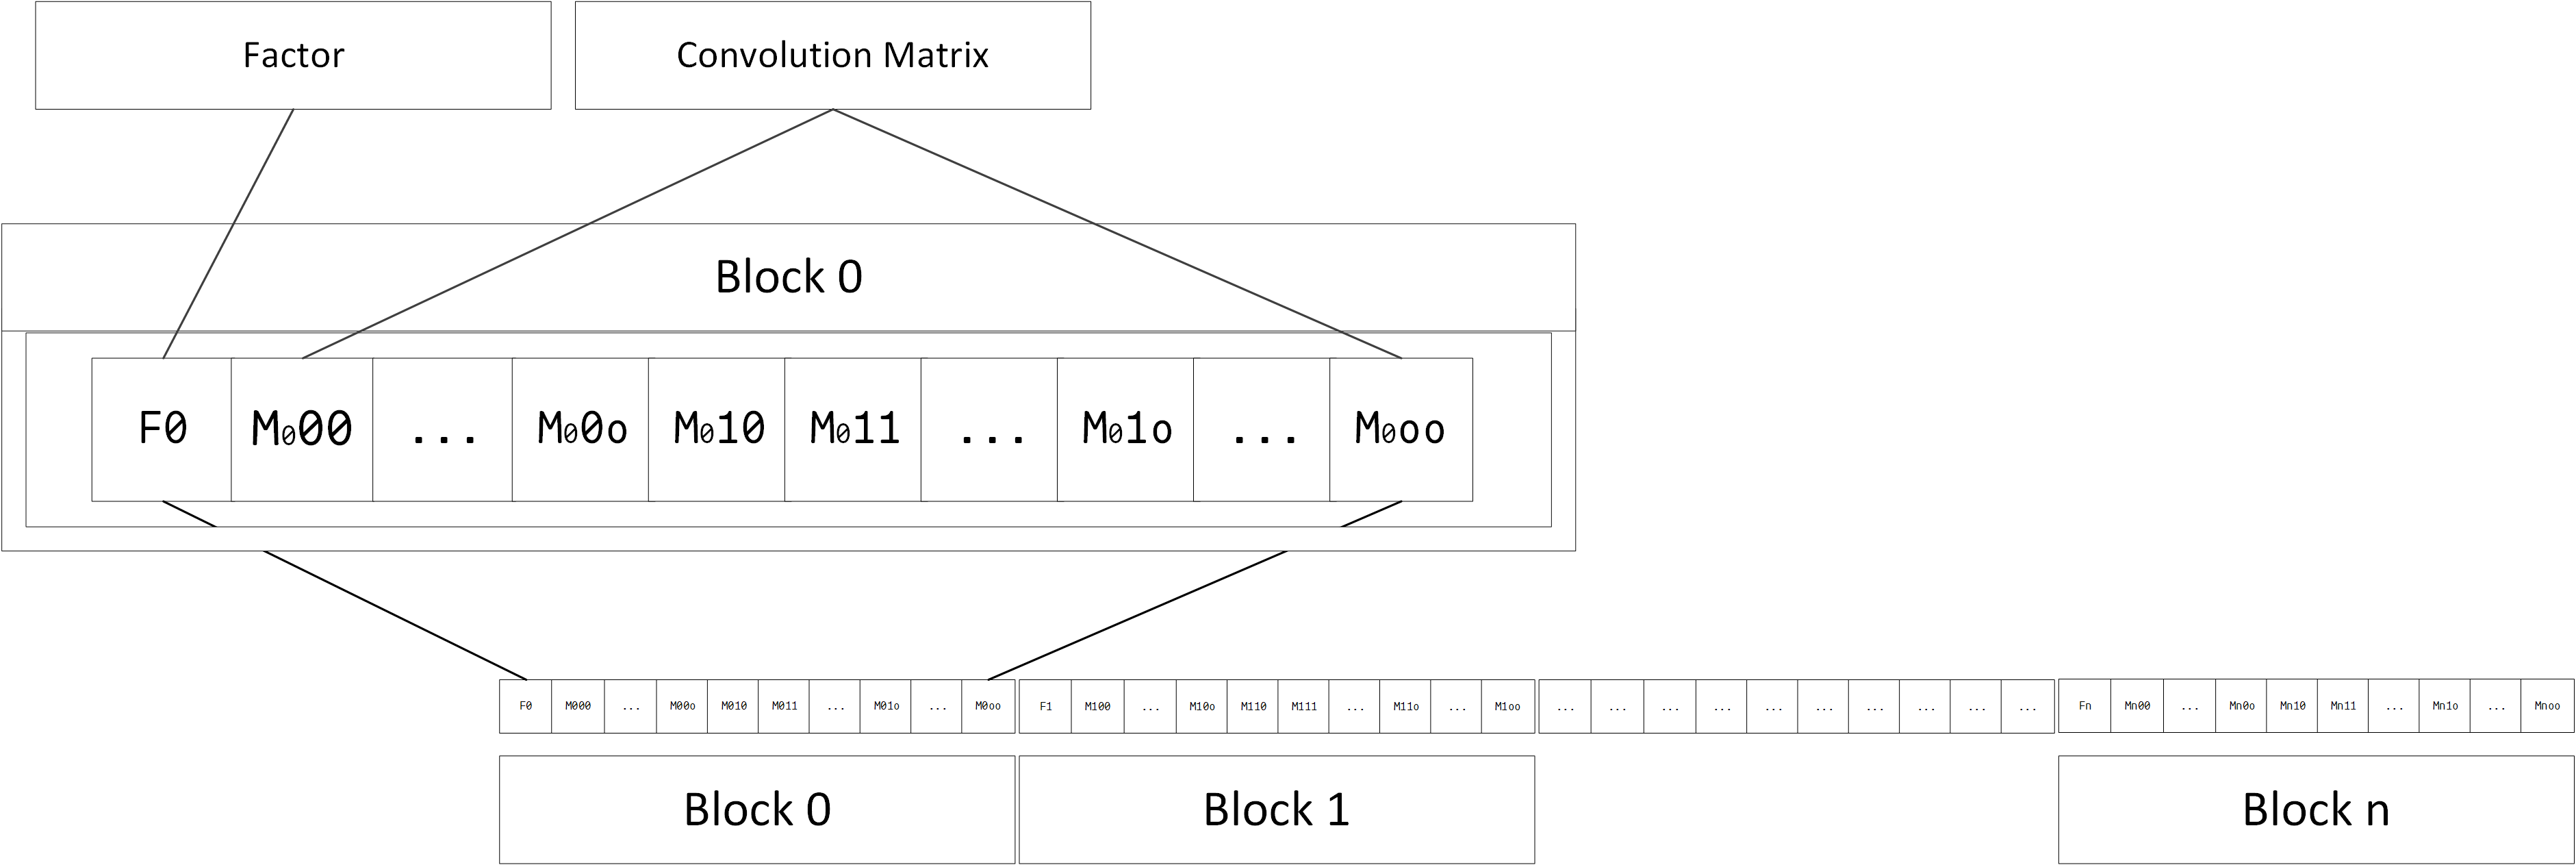
\includegraphics[scale=0.49]{Figuras/VetorAtributosForecast-Ingles.png}
	\caption{Vetor de atributos do país.}
	\label{fig:VetorAtributosForecast-Ingles}
\end{figure}


\subsection{Implementando a Função de Avaliação}
\label{Implementando a Função de Avaliação}

Voltando então para a implementação da função de avaliação, com o número de dimensões e a estrutura do vetor de atributos dos países já definidos, pode-se então, definir a implementação da função de avaliação em três partes como descrita anteriormente, porém agora mais resumidamente e com foco na implementação de cada item:

\begin{itemize}
\item Tradução do vetor de atributos dos países;
\item Processamento dos mapas de previsão 
\begin{itemize}
\item Cálculo parcial do erro;
\end{itemize}
\item Avaliação dos erros e atribuição do custo;
\end{itemize}

A tradução do vetor de atributos deve gerar dois elementos, o vetor de ponderações e o vetor de máscaras. Ambos são obtidos em um mesmo bloco que itera \emph{i} de 0 até o número de ponderações \emph{PonderationCount}. Assim o vetor de ponderações é preenchido como \ref{eq:forecastPonderation}:
	
\begin{equation}
\label{eq:forecastPonderation}
\begin{split}
ponderations[i] = element.Attributes[ponderationIndex];\\
\text{Sendo}\\
ponderationIndex = i \cdot (maskCount + 1);
\end{split}
\end{equation}


Em \ref{eq:forecastPonderation} ocorre uma cópia do valor contido no vetor de atributos no índice \emph{ponderationIndex} para o índice \emph{i} do vetor \emph{ponderations}.

E em seguida, utilizando-se deste índice de ponderações \emph{ponderationIndex}, copiam-se um intervalo de valores do vetor de atributos do país, de modo que esta cópia comece no índice \emph{ponderationIndex + 1} deste valor de atributos, que representa o primeiro elemento da máscara, e copie os valores até se atingir uma quantidade de elementos igual a \emph{maskCount}, tendo assim, um vetor de elementos que represente a máscara. Ainda não se tem portanto, a máscara no formato de uma matriz, então chama-se uma função externa para converter um vetor unidimensional de valores para uma matriz que represente uma máscara ou filtro de convolução, respeitando a ordem da máscara, como mostra o exemplo contendo o algoritmo \ref{alg:CountryTransform} usado em tal transformação:

\vspace{10px}
\begin{algorithm}[h]
\SetAlgoLined
\KwData{
\\ Atributos - [1, 2, 3, 4, 5, 6, 7, 8, 9].
\\ Ordem - 3.
}
\KwResult{ 

\\Máscara\\
[1, 2, 3]\\
[4, 5, 6]\\
[7, 8, 9]

}
inicializar a matriz \emph{masks[Ordem][Ordem]} com zeros\;

\For{$k \leftarrow $0 \KwTo $Ordem*Ordem$}
{
\tcp{índice x é o resto da divisão de k por ordem.}
x = k \% Ordem\;
\tcp{índice y.}
y = (k - x ) / Ordem\;
mask[x][y] = Atributos[k]\; 
}
\caption{ Algoritmo Transformação do vetor de atributos do país.}
\label{alg:CountryTransform}
\end{algorithm}

Após a obtenção da máscara representada pela estrutura matricial, que é então adicionada em um vetor de matrizes chamado \emph{ponderationMasks}, termina-se a etapa de tradução do vetor de atributos do país para dois vetores, \emph{ponderations} e \emph{ponderationMasks}, contendo os valores de ponderação e as máscaras de convolução usadas para gerar os mapas de ponderação respectivamente.

Seguindo, para a etapa de processamento dos mapas de previsão, diversas inicializações são feitas, na ordem:
\begin{enumerate}
\item Inicializar o vetor de valores resultados em \emph{resultValues}.
\item Inicializar o vetor de imagens resultado da operação de ponderação entre as matrizes de convolução em \emph{ponderationImages}.
\item Inicializar o vetor de mapas resultantes da convolução em \emph{resultMaps}
\item Inicializar uma matriz para representar o mapa final gerado dos processos de convolução e ponderação, para posterior comparação e cálculo do erro.
\end{enumerate}



Após estas atualizações, itera-se por todos os mapas com exceção do último, gerando os mapas de convolução de cada período, no vetor \emph{resultMaps}, mapeando o resultado do cálculo para um mapa ponderado, na matriz \emph{result} , e gerando então, um mapa final, \emph{finalResult}, de previsão do próximo período ao se somar o mapa do período atual. E, por fim, comparando  ambos, o mapa real do próximo período e o mapa final de previsão processado, a fim de gerar os erros e armazená-los no vetor \emph{resultValues} para posterior definição de custo do país, conforme mostra o algoritmo:

\vspace{10px}
\begin{algorithm}[h]
\SetAlgoLined
\KwData
{
\\ \emph{PonderationCount} - número de ponderações.
\\ \emph{TrainingSize} - quantidade de períodos para treino.
\\ \emph{height} - altura em quadrículas da região.
\\ \emph{width} - largura em quadrículas da região.
\\ \emph{MapList} - Lista de mapas históricos de quadrículas.
\\ \emph{masks} - vetor de máscaras de convolução.
\\ \emph{ponderations} - vetor de fatores de ponderação. 
}
\KwResult{ \\ cost - custo avaliado do país. }

next = 1\;
\tcp{Iteração de previsão.}
\For{$now \leftarrow $0 \KwTo $TrainingSize - 1$}
{
\tcp{Início da função de previsão.}
	\For{$i \leftarrow $0 \KwTo $PonderationCount$}
    {
    	resultMaps[i] = Convolution(MapList[now].MapMatrix, masks[i])\;
    }
    result = new Matrix[width][height]\;
    \For{$x \leftarrow $0 \KwTo $width$}
    {
    	\For{$y \leftarrow $0 \KwTo $height$}
        {
          num = 0; den = 0\;
          \For{$i \leftarrow $0 \KwTo $PonderationCount$}
          {
			num += resultMaps[i].MapMatrix[x][y] * ponderations[i]\;
            den += resultMaps[i].MapMatrix[x][y]\;
          }
          result[x][y] = num / den\;
        }
    }
    finalResult = Sum(MapList[now].MapMatrix, result)\;
    \tcp{End Of Fp function.}
    resultValues[now] = Diference(MapList[next].MapMatrix, finalResult) * 0.5 + Abs(Diference(MapList[now].MapMatrix, finalResult) - absoluteGrowths[now]) * 0.5\;
    next = now + 1;
}
cost = resultValues.Sum()\;
\caption{ Avaliação do país.}
\label{alg:CountryEval}
\end{algorithm}

Na linha 1 inicia-se o valor de iteração para o índice do próximo período em \emph{next}. Na linha 2 inicia-se o processo de treino do país, passando por todos os períodos exceto o último, de forma que se itere o valor \emph{now}, que representa o período atual, até um período antes do último. Em seguida, nas linhas 3 e 4, geram-se todos os mapas de convolução, referentes a cada ponderação, baseando-se no mapa matriz do período definido por \emph{now}. A linha 6 apenas inicializa um mapa vazio com as mesmas dimensões dos mapas matrizes dos períodos. Então, nas linhas 7 e 8, inicia-se o processo de iteração por todas as quadrículas (ou pixels) do mapa matriz, usando \emph{x} para deslocamento pela largura e \emph{y} pela altura. Em 10, 11, 12 calcula-se a soma dos numeradores e denominadores das ponderações de cada mapa multiplicado pelo valor de ponderação, gerando assim, um valor ponderado para cada pixel dentre cada um dos mapas de ponderações. Deste modo, atribui-se ao pixel \(\left(x,y\right)\) na matriz resultado, o valor ponderado \emph{result[x][y]}, sendo o numerador dividido pelo denominador calculado no passo anterior usando os valores de ponderação como base de cálculo. Para a obtenção do mapa final de previsão na linha 17, adiciona-se o mapa resultado ao mapa base do período, sendo que tal mapa final represente o mapa futuro como sendo o mapa atual somado com os valores de desvio gerados da ponderação das convoluções de cada pixel. Por fim, na linha 18, ocorre a atribuição do valor de erro gerado pela previsão deste período para o vetor \emph{resultValues}, sendo esta a parte mais crítica, que define de fato se a previsão feita é semelhante ao esperado ou não.

Observa-se que o cálculo dos valores \emph{resultValues} são ponderados com \(0.5\) e \(0.5\), o que indica que ambos os valores têm mesmo peso para a avaliação. Caso fosse utilizado \(0.75\) para a previsão e \(0.25\) para os valores absolutos, teria-se uma avaliação que 'prefere’ que o país tenha suas matrizes de convolução e fatores de ponderação se caracterizando mais nos mapas matrizes reais do que levando em consideração os crescimentos absolutos entre os períodos previstos e reais. 

Em seguida, os erros acumulados no vetor \emph{resultValue}, referentes cada um a uma iteração pelos períodos, comparando-os ao período seguinte, devem ser somados e então atribuídos como custo do país, terminando assim a avaliação do país, como:

\[Country.Cost = Sum(resultValues);\]

As funções \emph{Abs}, \emph{Sum}, \emph{Diference} e \emph{Convolution}, são funções, chamadas externamente, que operam valores, vetores ou, matrizes, tal que:
\begin{itemize}
\item \emph{Abs} recebe um valor numérico e retorna o valor absoluto deste número.
\item \emph{Sum} tem duas sobrecargas, sendo
\begin{itemize}
\item a primeira, tendo como entrada um vetor de valores e retorna a soma entre todos os valores deste vetor.
\item e a segunda, tem como entrada duas matrizes de largura e altura iguais e retorna como resultado uma nova matriz, com altura e largura também iguais Às matrizes de entrada, onde esta matriz resultado representa a soma dos elementos de cada índice das matrizes de entrada.
\end{itemize}
\item \emph{Diference} tem como entrada duas matrizes de altura e largura iguais, onde será calculada e retornada a diferença total e absoluta entre os os elementos de cada índice das matrizes de entrada.
\item \emph{Convolution} é uma operação mais complexa, que executa a convolução de um filtro ou matriz de convolução sobre uma matriz, ambos passados como parâmetro, e neste caso, ignora-se os valores de ajuste(\emph{offset}) e divisor (citados nos conceitos de convolução) são mantidos nulos, valendo respectivamente 0 e 1, uma vez que o ICA já se encarrega de configurar apropriadamente os índices da matriz, como se ela já possuísse os valores de ajuste e divisor aplicados a si.
\end{itemize}

A avaliação ocorre para todos os indivíduos na mesma etapa, podendo ser processada em serial ou em paralelo. Observe que a avaliação de cada indivíduo ocorre independente dos demais, de modo que todo recurso compartilhado não restrinja o uso apenas para aquela avaliação, possibilitando assim que o processamento das avaliações dos países possa ser executado em tarefas paralelas. Assim que todas as avaliações são finalizadas, independente de terem ocorrido paralela ou serialmente, o ICA passa para as próximas etapas que, então irão alterar todas as características dos países até que se termine a iteração e entre novamente na etapa de avaliação, onde todos os indivíduos são novamente avaliados. A condição de parada padrão geralmente é o número máximo de décadas, que quando atingida, termina a evolução dos indivíduos e consequentemente da competição imperialista. 



\section{Aplicando Função de Previsão}
\label{A Etapa de Previsão}

No fim da competição imperialista o método \(Run()\) acaba sua execução retornando para o escopo da aplicação, sendo agora possível obter qualquer país usado na competição imperialista, e utilizá-lo para aplicar tal solução ao problema. O interessante é utilizar o país de menor custo, uma vez que esta é a melhor solução buscada pelo ICA. Então, este melhor indivíduo é usado na etapa de teste, que, neste caso, é aplicado para gerar mapas de previsão de períodos futuros através de um processo muito semelhante ao processo feito pela função de avaliação. No processo de avaliação, iterou-se por diversos períodos gerando um mapa de previsão para cada período. No caso da etapa de testes, não se faz tal iteração, apenas executa-se o processo de geração do mapa de previsão, que basicamente faz os processos:

\begin{itemize}
	\item Tradução do vetor de atributos do país.
	\item Processamento de mapas de previsão a partir do último período usado.
\end{itemize}

O processo de tradução do vetor de atributos do país já fora detalhado anteriormente e não muda em nada durante esta etapa de testes. O processamento de um mapa de previsão deve sempre ocorrer a partir do último mapa usado na etapa de avaliação, sendo este o ano base para que se gere as demais previsões. Este processo de testes sempre irá gerar um período de previsão a frente do período passado, então para se gerar mais de um período de previsão, é necessário executar este processo tantas vezes quanto se queira ter previsões de períodos futuros, passando como parâmetro, um mapa para previsão e um país, para se gerar um segundo que é o resultado do processo de previsão usando o método de convoluções ponderadas, como mostra o algoritmo \ref{alg:Fp}:

\begin{algorithm}[h]
	\SetAlgoLined
	\KwData
	{
		\\ \emph{PonderationCount} - número de ponderações.
		\\ \emph{Map} - o mapa base, que terá previsão de 1 período à frente.
		\\ \emph{height} - altura em quadrículas da região.
		\\ \emph{width} - largura em quadrículas da região.
		\\ \emph{masks} - vetor de máscaras de convolução.
		\\ \emph{ponderations} - vetor de fatores de ponderação. 
	}
	\KwResult{ \\ finalResult - como o mapa de previsão de 1 período à frente de Map. }
	
	\For{$i \leftarrow $0 \KwTo $PonderationCount$}
	{
		resultMaps[i] = Convolution(Map.MapMatrix, masks[i])\;
	}
	result = new Matrix[width][height]\;
	\For{$x \leftarrow $0 \KwTo $width$}
	{
		\For{$y \leftarrow $0 \KwTo $height$}
		{
			num = 0; den = 0\;
			\For{$i \leftarrow $0 \KwTo $PonderationCount$}
			{
				num += resultMaps[i].MapMatrix[x][y] * ponderations[i]\;
				den += resultMaps[i].MapMatrix[x][y]\;
			}
			result[x][y] = num / den\;
		}
	}
	finalResult = Sum(Map.MapMatrix, result)\;
	
	\caption{Algoritmo função de previsão}
	\label{alg:Fp}
\end{algorithm}

Observe que o algoritmo é uma cópia de uma parte da função de avaliação, que gera o mapa de previsão de apenas um período, fazendo a soma de todos os mapas operando-os pela convolução e ponderando-os em um mapa final. Assim, como mencionado anteriormente, é possível gerar várias previsões, utilizando o mapa gerado de uma previsão t1` para se prever t2` e assim por diante. Porém, como a previsão de um segundo período é sobre uma previsão já feita, acumulam-se os erros de previsões, aumentando drasticamente a incerteza para previsões mais futuras.

Com esta função de previsão é possível então gerar mapas futuros de um período à frente de um histórico de mapas separados por períodos homogêneos. Pode-se ainda gerar a previsão de mais períodos futuros, utilizando-se dos mapas previstos gerados pela própria função de previsão, reinseridos como mapa base para a previsão de mais um período futuro, porém, ao repetir tal processo diversas vezes propaga-se muito os erros gerados nas primeiras previsões, fazendo com que cada período extra aumente a incerteza da previsão. 

É interessante notar que a função de previsão será chamada diversas vezes para a previsão de apenas um mapa, sendo uma vez para cada região de quadrículas do mapa. Ou seja, cada região tem seus parâmetros de previsão otimizados pelo ICA e o parâmetro base como sendo a própria região de quadrículas. Assim, o P.E.M.D. deve fazer uma chamada da função previsão para cada região, obtendo assim diversas previsões das regiões separadamente, e por fim, deve ser capaz de recriar o mapa final de previsão composto de todas as regiões previstas.





